%!TEX program = lualatex

\documentclass{beamer}

\usepackage{fontspec}
\usepackage{libertine}
\usepackage{microtype}
\usepackage{amssymb}
\usepackage{mathtools}
\usepackage{unicode-math}
\usepackage{lualatex-math}

\setmainfont[Ligatures=TeX]{Linux Biolinum O}
\setmathfont[math-style=ISO,bold-style=ISO,vargreek-shape=TeX,Ligatures=TeX]{TeX Gyre Pagella Math}

\usepackage{polyglossia} % babel replacement for use with fontspec
\setdefaultlanguage[variant=american]{english}
\selectlanguage[variant=american]{english}
\usepackage{csquotes}
\usepackage[load-configurations={abbreviations,binary}]{siunitx}
\sisetup{load-configurations = abbreviations,binary-units}

\usetheme{EastLansing}
\usecolortheme{seagull}
\useinnertheme{rectangles}
\usefonttheme{professionalfonts}



\usepackage[defernumbers=true, style=alphabetic, citestyle=alphabetic, firstinits=true, backend=biber, doi=true, url=true, block=ragged, maxnames=6]{biblatex}
\addbibresource{../../bibliography/common.bib}
\addbibresource{../../bibliography/rfc-shorthands.bib}
\addbibresource{../../bibliography/3gpp.bib}
\addbibresource{../../bibliography/mobile.bib}
\addbibresource{../../bibliography/video.bib}
\addbibresource{../../bibliography/network.bib}
\addbibresource{../../bibliography/crosslayer.bib}


\title[]{Evaluating Reliable Streaming in Mobile Networks}
\subtitle{Dissertation Presentation}
\author{Florian Metzger}
\institute[University of Vienna]
{
	University of Vienna\\
	Faculty of Computer Science\\
	Future Communication Research Group

}
\date[]{2015/01/XX}

%\subject{Informatik}

\begin{document}


\frame{\titlepage}

\begin{frame}
	\frametitle{Outline}
	\tableofcontents
\end{frame}

%%%%%%%%%%%%%%%%%%%%%%%%%%%%%%%%%%%%%%%%%%%%%%%%%%%%%%%%%%%%%%%%%%%%%%%%%%%%%%%%
\section{Introduction}
%%%



\begin{frame}
	\frametitle{Introduction}
\end{frame}

\begin{frame}
	\frametitle{Introduction}
\end{frame}

\begin{frame}
	\frametitle{Introduction}

	\begin{figure}
	\centering
	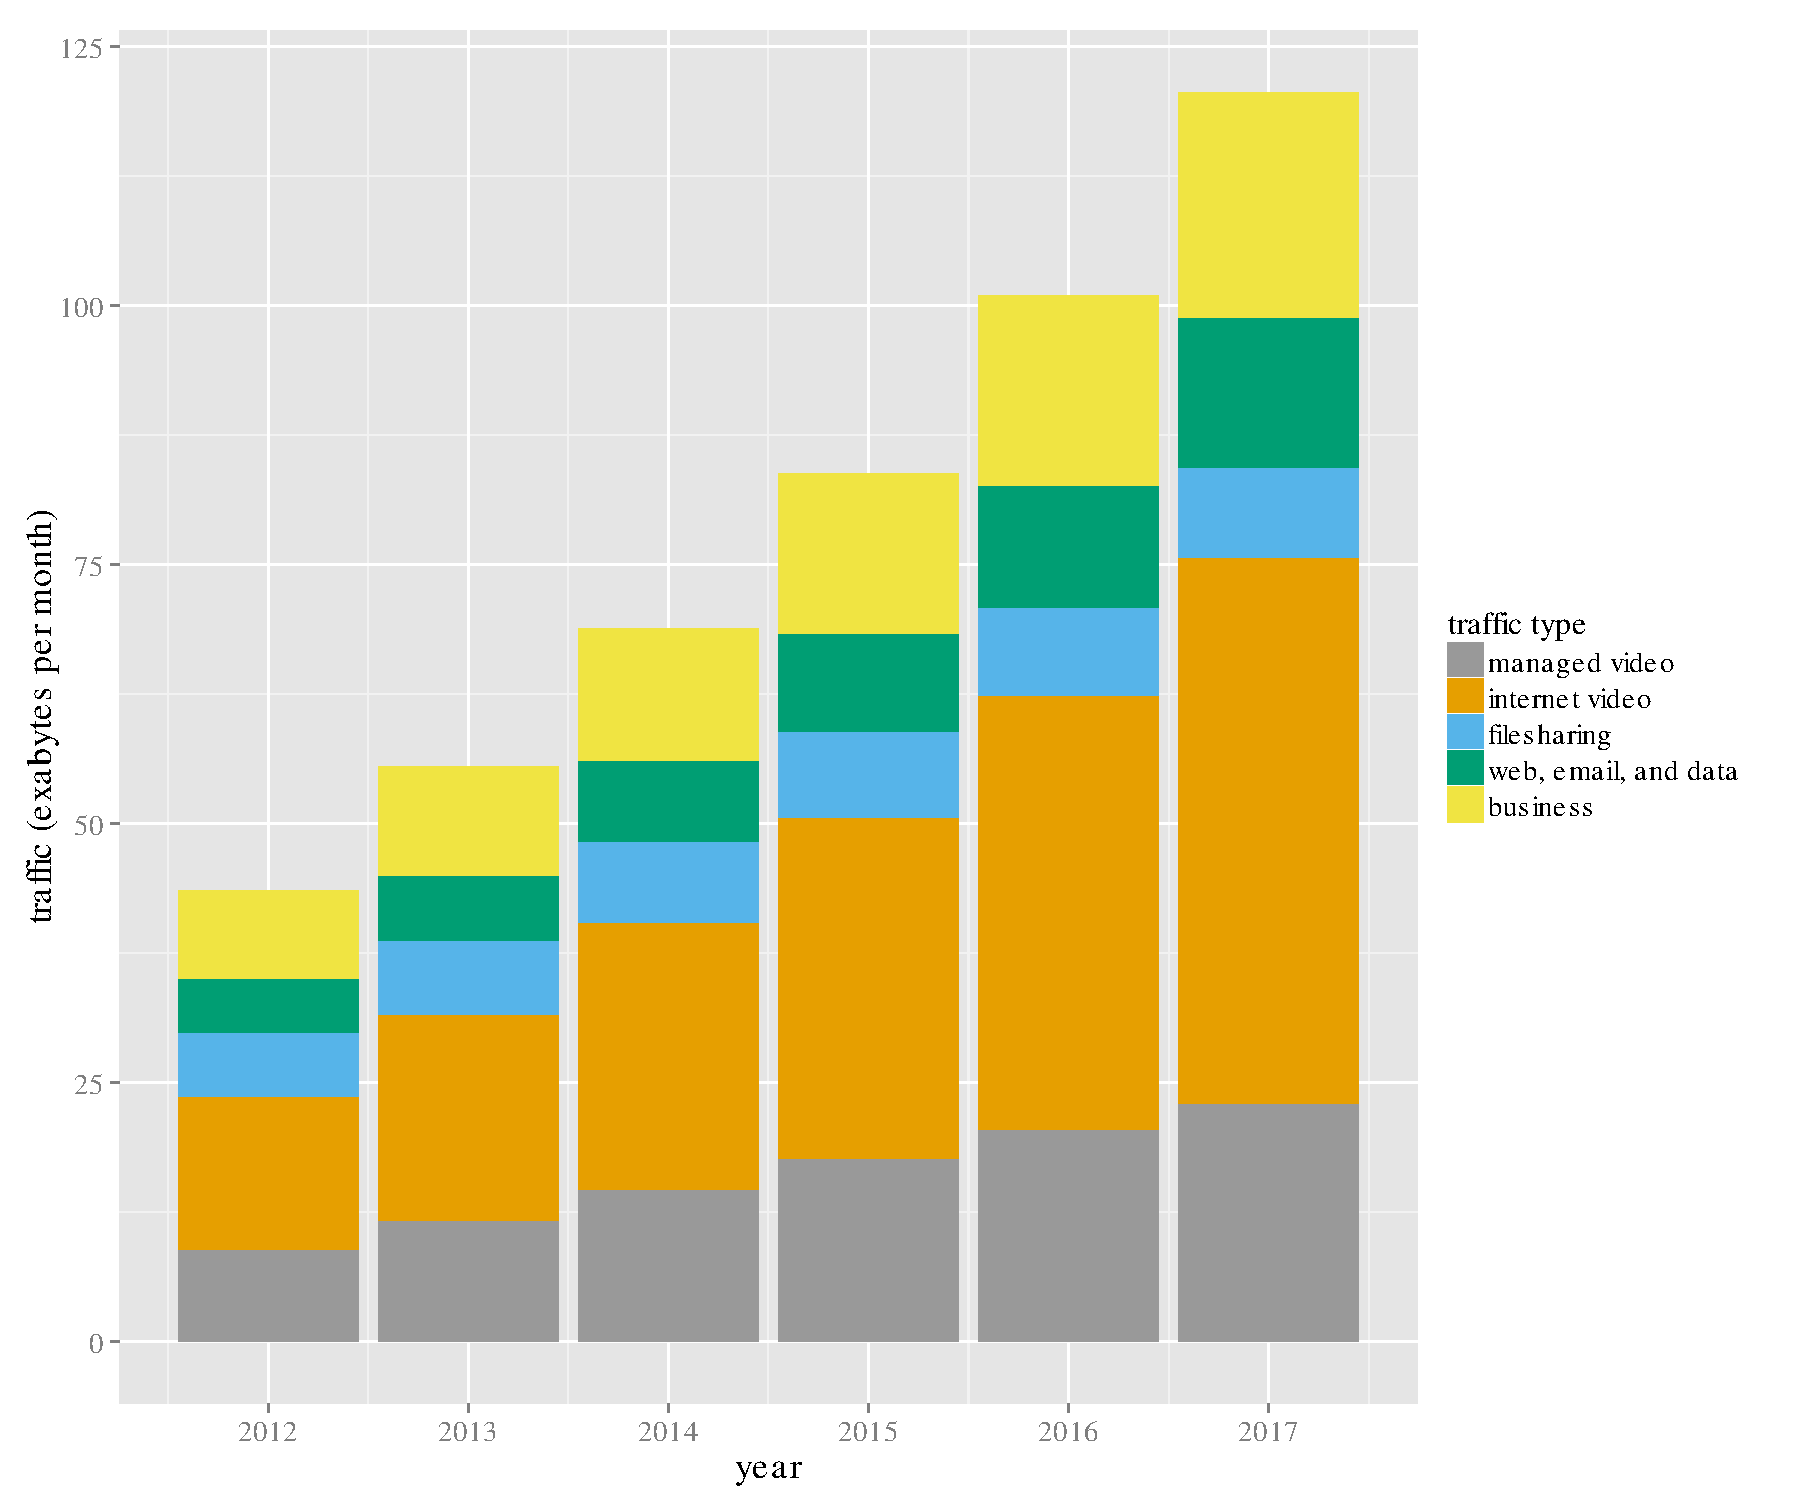
\includegraphics[height=6cm]{../../chapters/01-intro/images/r-cisco-vni-2013.pdf}
	\caption{Cisco's global consumer Internet traffic prediction (data source:~\cite{cisco2013VNI}).}
	\end{figure}
\end{frame}


\begin{frame}
	\frametitle{Thesis Parts}

	Thesis consists of two intersecting angles
	\begin{enumerate}
		\item Investigation of TCP-based video streaming techniques
			\begin{itemize}
				\item Protocol survey and classification
				\item Deriving a model
				\item Measurements with the model
			\end{itemize}
		\item Evaluation of a 3G core network
			\begin{itemize}
				\item Investigation and evaluation of the control plane
				\item \textbf{Modeling and simulating load}
			\end{itemize}
		\item Measuring video streaming in a 3G network 
	\end{enumerate}

	Presentation based on MMB'14 submission \textit{``A PDP Context Load Model and Virtualization
Gain for a Mobile Network's GGSN''}

	% \begin{block}{}
	% 	This presentation
	% \end{block}
\end{frame}



\begin{frame}
    \frametitle{Motivation}



	Mobile network planning and dimensioning today
    \begin{itemize}
    	\item based on expected user traffic
		\item good algorithms and tools for placing radio towers and planning radio propagation
		\item core network and control plane usually not given much consideration
	\end{itemize}

	Our approach
	\begin{itemize}
		\item presents queuing models for a GGSN in the core network
		\item models simulated with data from a real network
		\item can be used to dimension for control plane
		\item offers more scaling options
	\end{itemize}

\end{frame}



%%%%%%%%%%%%%%%%%%%%%%%%%%%%%%%%%%%%%%%%%%%%%%%%%%%%%%%%%%%%%%%%%%%%%%%%%%%%%%%%
\section{Reliable Streaming Models}
%%%

\begin{frame}
	\frametitle{Introduction}
\end{frame}


\begin{frame}
	\frametitle{Streaming Categorization}
\end{frame}


\begin{frame}
	\frametitle{Reliable Streaming}

	Pure Progressive
	Segmented
	Adaptive

	Stalling as sole quality metric
\end{frame}



\begin{frame}
	\frametitle{Playback and Retrieval Strategies}

	Pure Progressive
	Segmented
	Adaptive
	\begin{figure}

	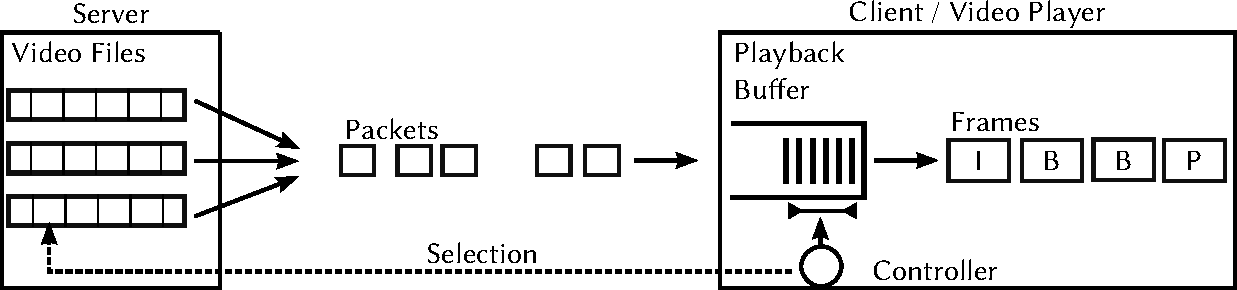
\includegraphics[height=2cm]{../../chapters/03-streaming/images/playback-model.pdf}
	\caption{Reliable streaming playback model based on buffer control.}
	\end{figure}

\end{frame}

\begin{frame}
	\frametitle{Playback Strategies Parameter Space}

	\begin{figure}
		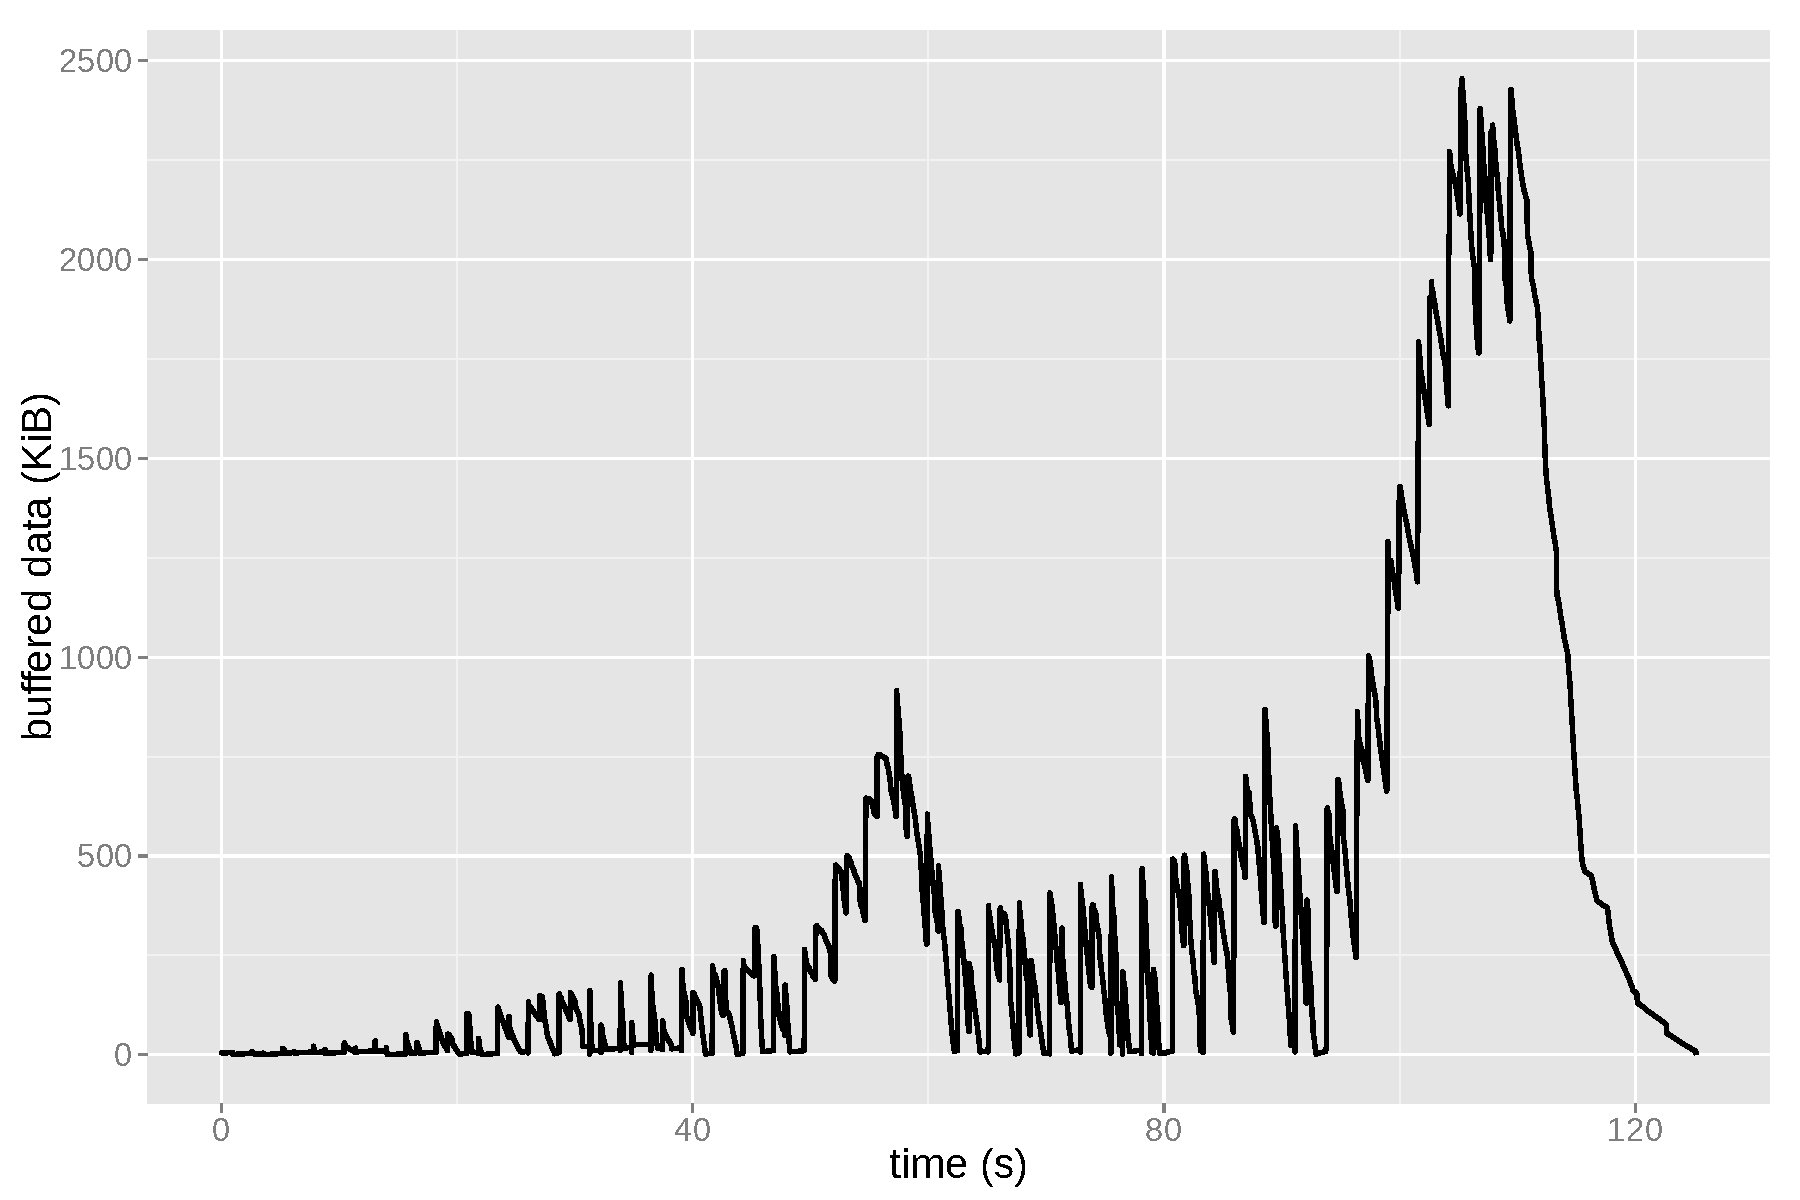
\includegraphics[height=4cm]{../../chapters/03-streaming/images/R-bufferlevel-stall.pdf}
		\caption{Buffer fill level with null strategy; \SI{33}{\second} total stalling.}
	\end{figure}

	\begin{figure}
		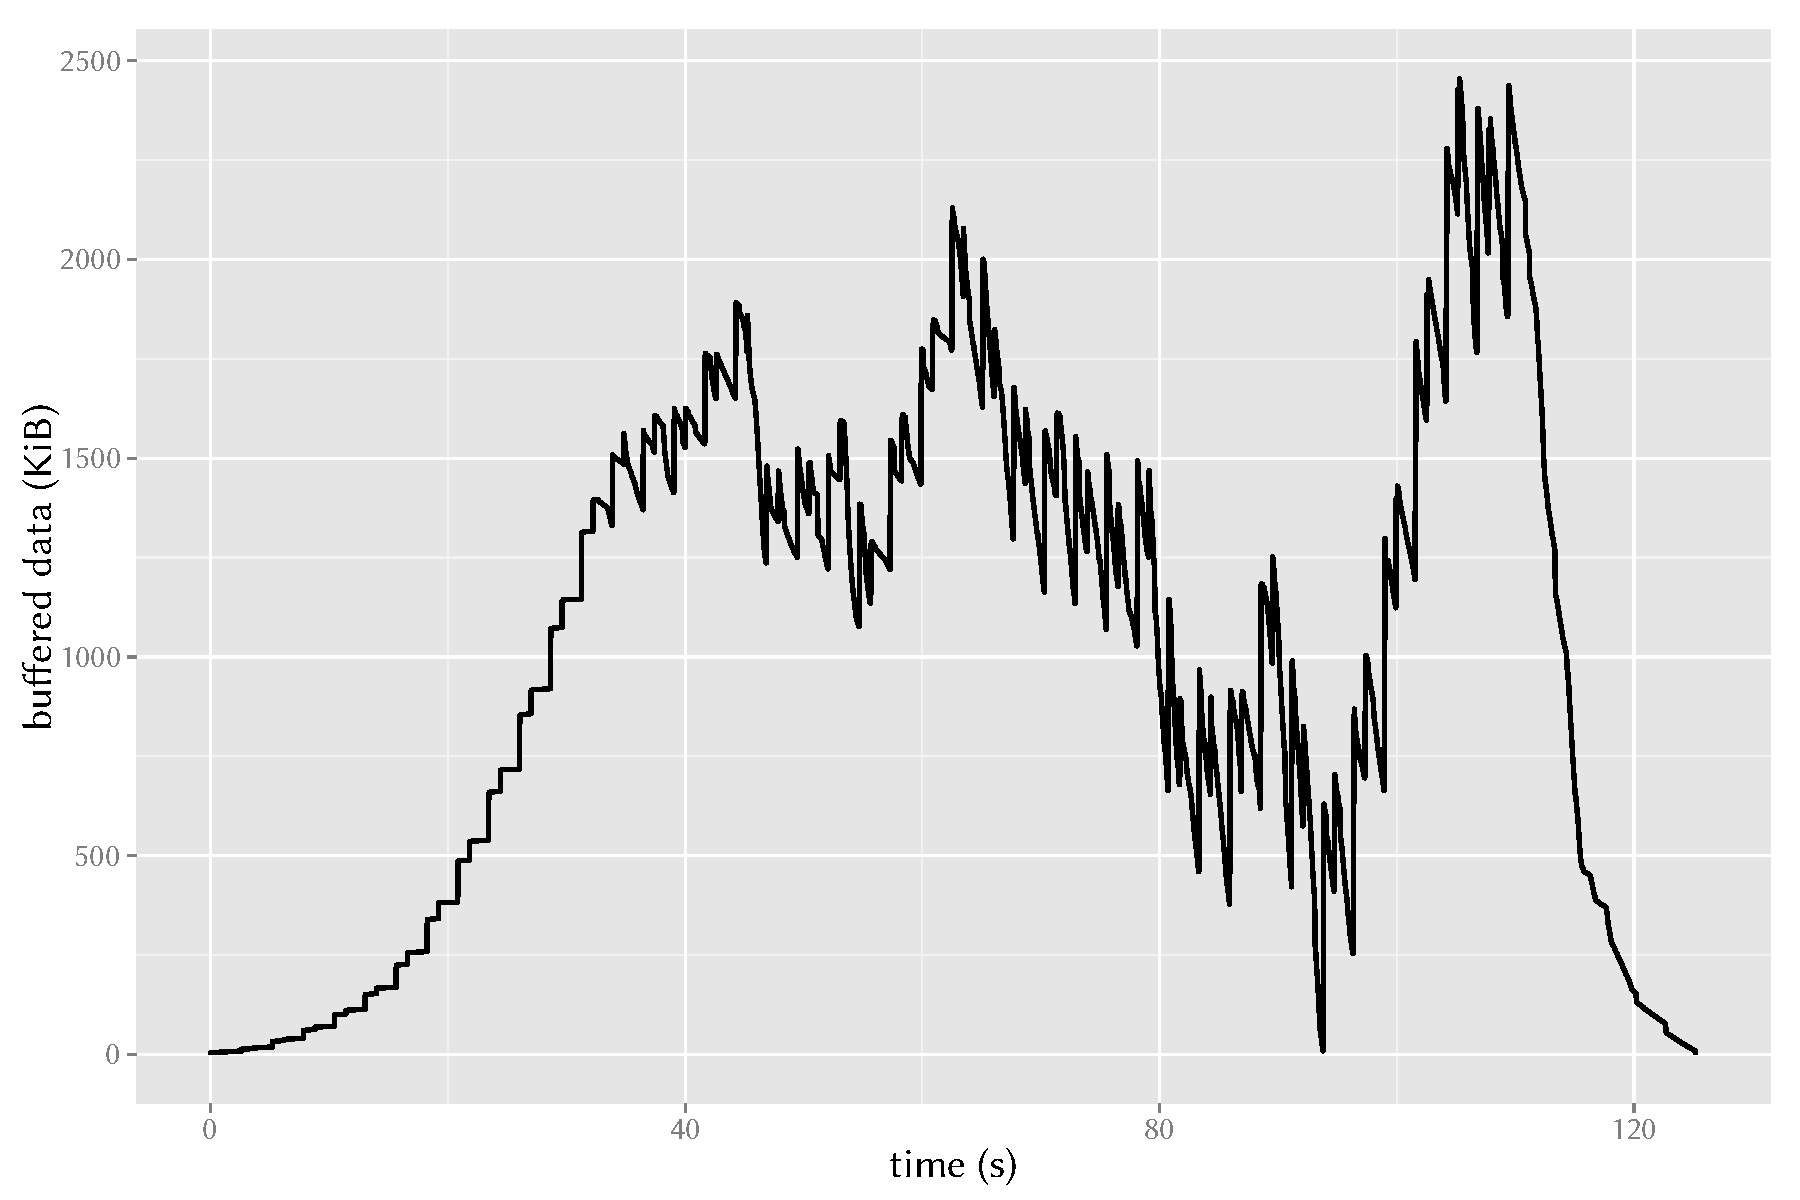
\includegraphics[height=4cm]{../../chapters/03-streaming/images/R-bufferlevel-startdelay.pdf}
		\caption{Sample Buffer fill level for the delayed playback predictive strategy, \SI{33}{\second} total stalling.}
	\end{figure}
\end{frame}


\begin{frame}
	\frametitle{Streaming Measurements}

	\begin{figure}
		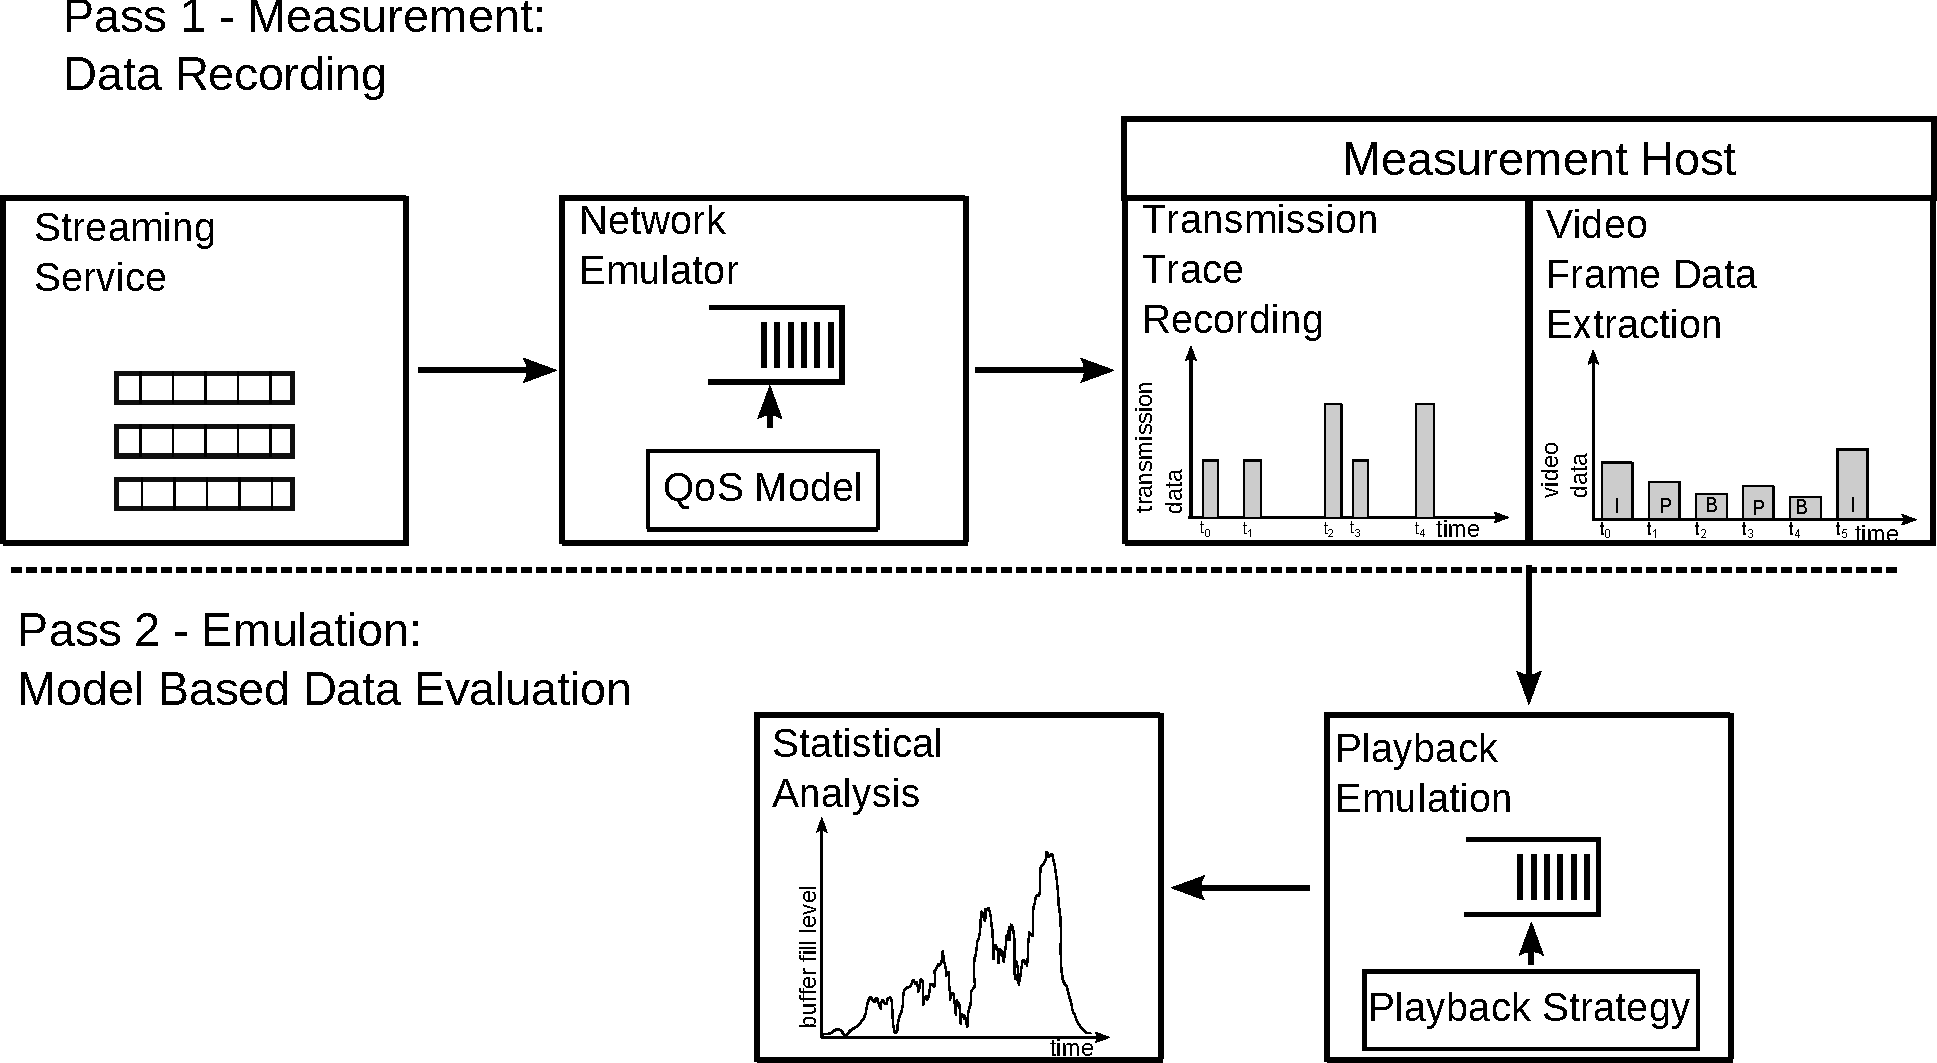
\includegraphics[height=4cm]{../../chapters/03-streaming/images/measurement-model.pdf}
		\caption{Overview of the measurement framework for progressive streaming playback strategies.}
	\end{figure}

\end{frame}



\begin{frame}
	\frametitle{Streaming Measurements: Latency}

	\begin{figure}
		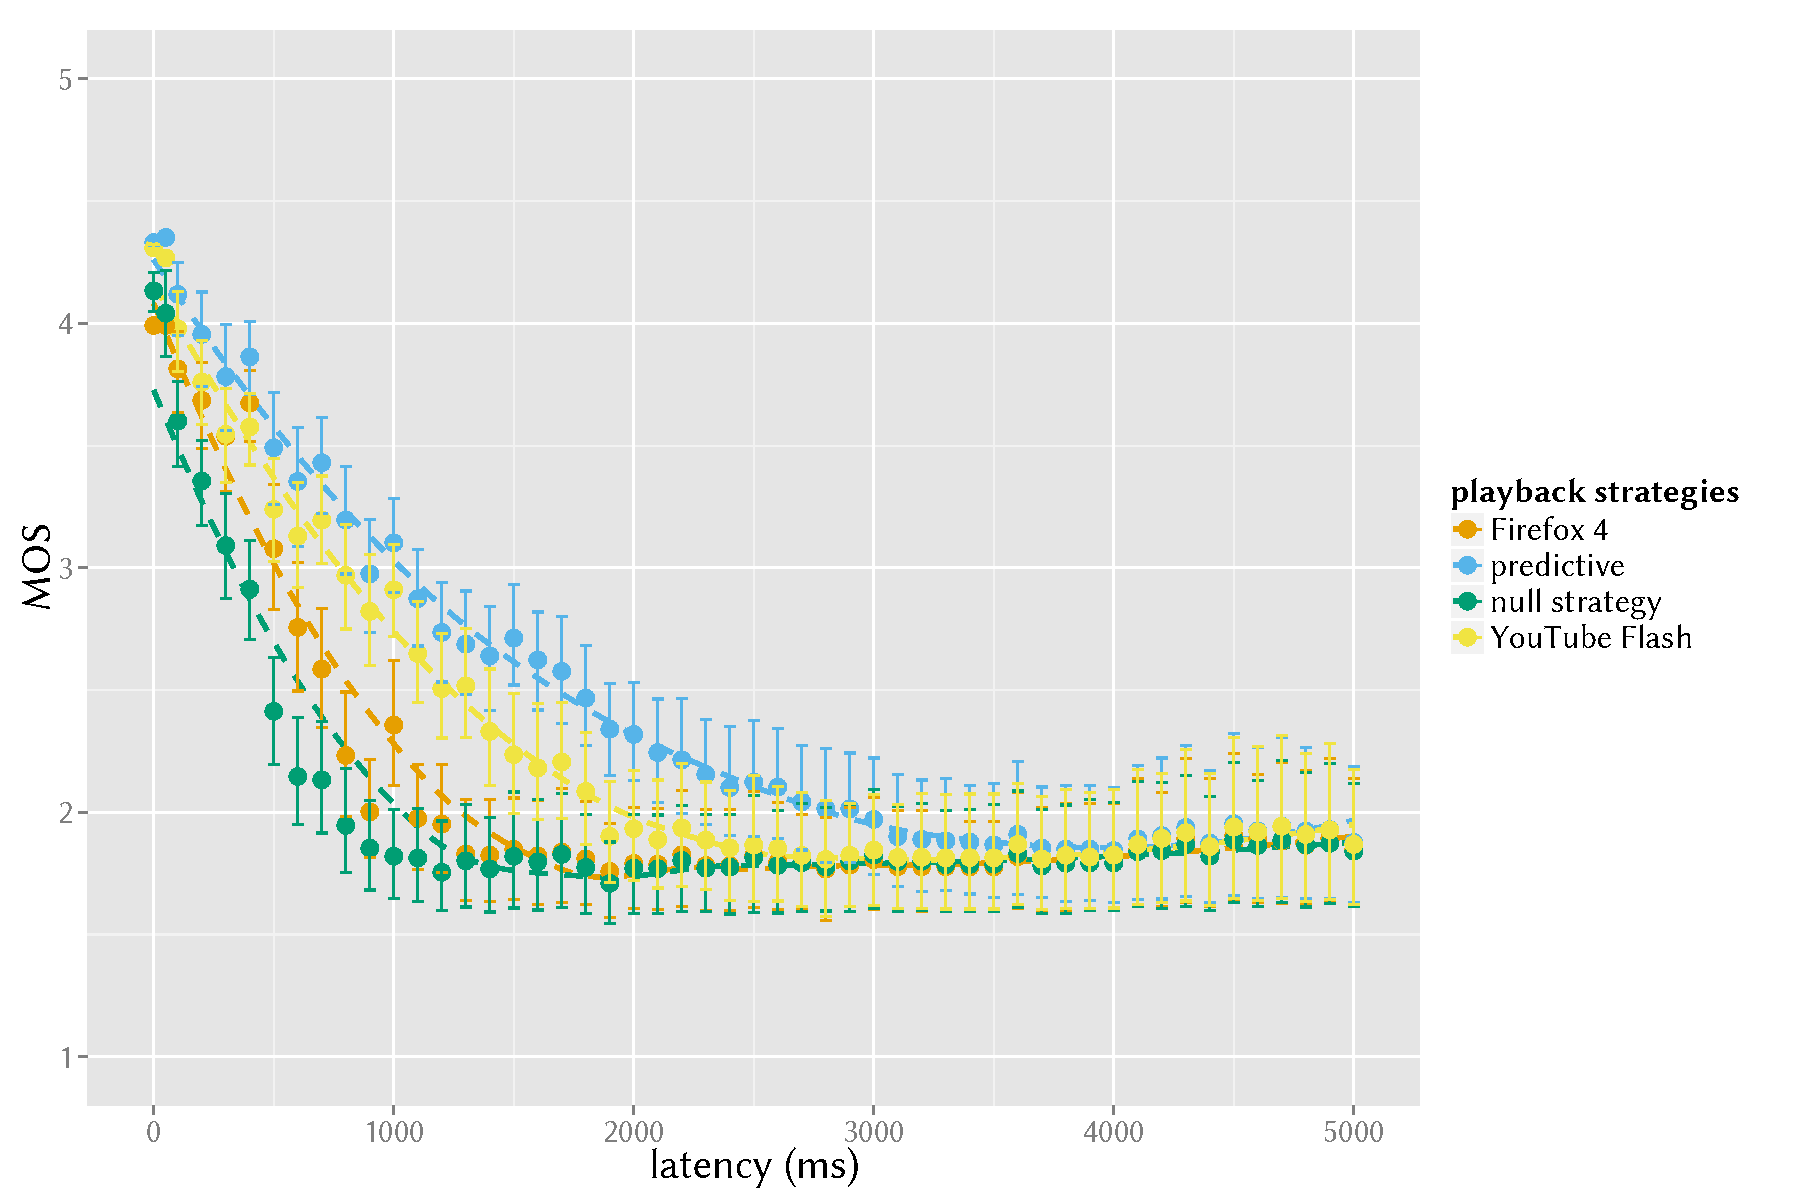
\includegraphics[height=4cm]{../../chapters/03-streaming/images/R-playbackemulation-qoe-latency.pdf}
		\caption{Calculated MOS for the latency measurement series.}
	\end{figure}


\end{frame}


%%%%%%%%%%%%%%%%%%%%%%%%%%%%%%%%%%%%%%%%%%%%%%%%%%%%%%%%%%%%%%%%%%%%%%%%%%%%%%%%
\section{Mobile Network Structures and Load Models}
%%%

\begin{frame}
	\frametitle{Introduction}
\end{frame}
\begin{frame}
    \frametitle{GTP Tunnels and Dataset}

      \begin{center}
		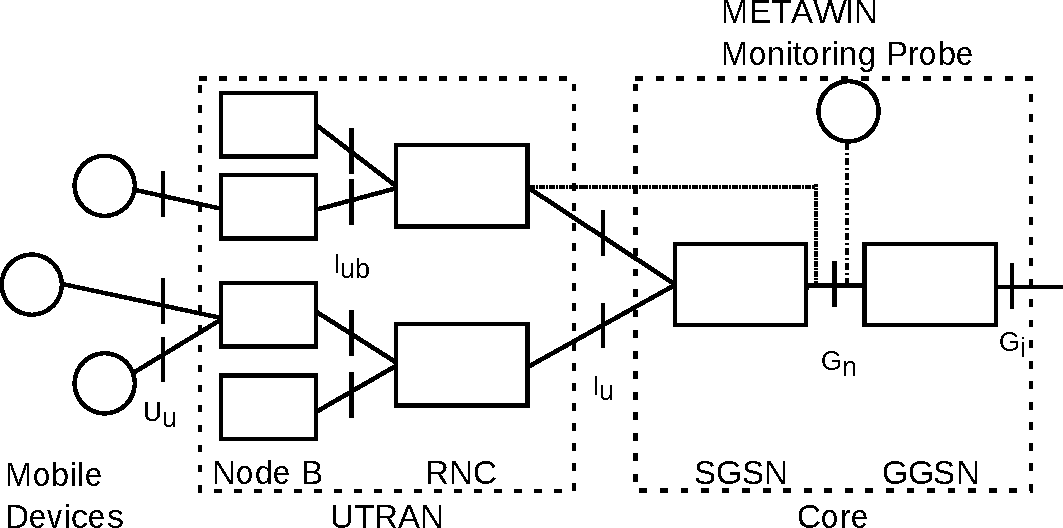
\includegraphics[height=3cm]{../../chapters/04-mobilenets/images/umts-network.pdf}
	\end{center}

	% \begin{center}
	% 	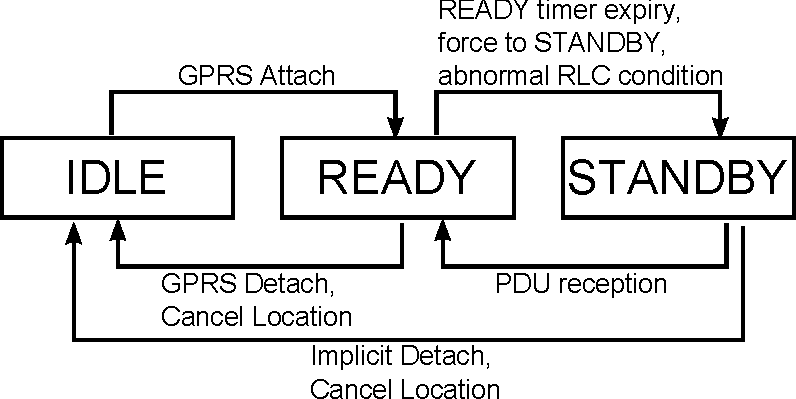
\includegraphics[height=2.5cm]{figures/mm-state-model.pdf}
 % 	\end{center}

	%Tunneling concept
    \begin{itemize}
		\item Any user traffic in a 3G net is encapsulated into tunnels
		\item GPRS Tunneling Protocol (GTP) used between SGSN and GGSN
		\item Tunnel state (PDP Context) held at and signaled between core nodes through create/delete/update messages
		%\item tunnel management signaling: creation, deletion, and update request/response messages
	\end{itemize}
	Recorded dataset
	\begin{itemize}
		\item One week long passive measurements in an operator's core network (METAWIN, April 2011)
		\item 2.2Bn anonymized user traffic records, 410M GTP tunnel management messages
	\end{itemize}
\end{frame}



\begin{frame}
	\frametitle{Tunnel Arrivals}
		%\framesubtitle{Interarrival Time of Successful Tunnel Requests}
	\begin{columns}[c]
		\begin{column}{6.5cm}
				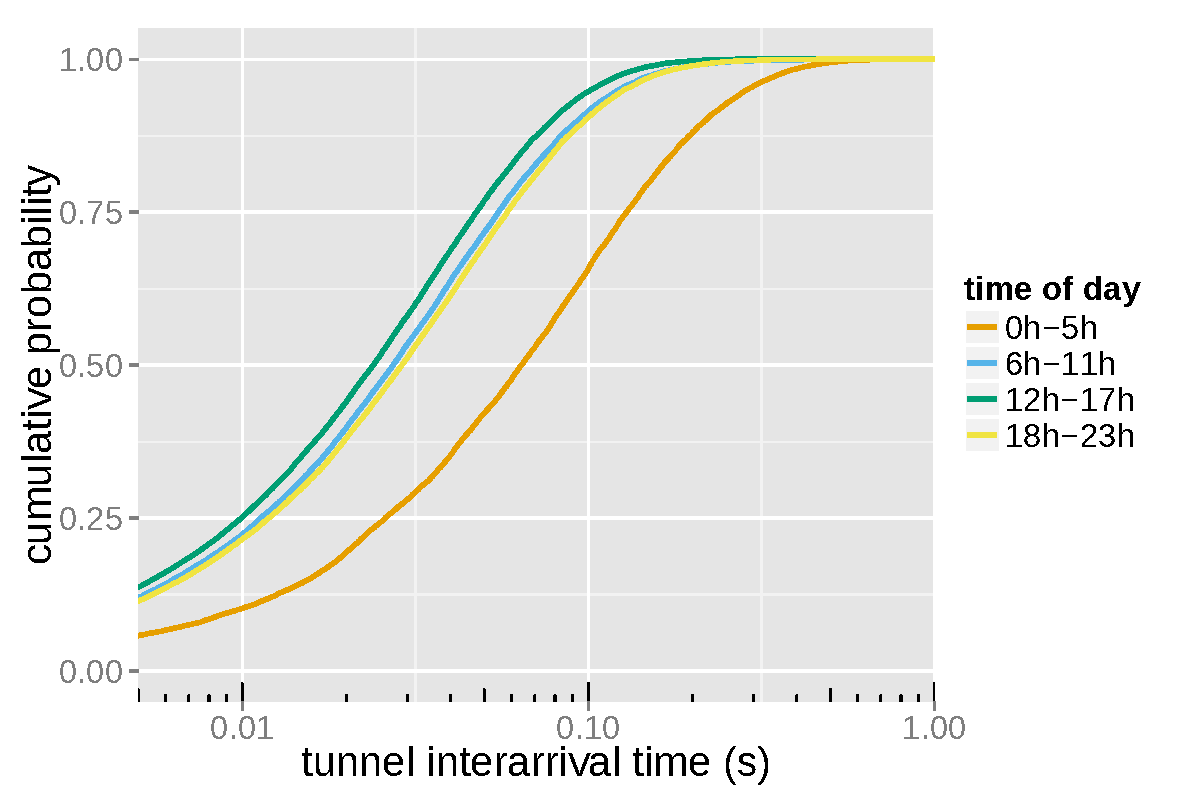
\includegraphics[width=6.5cm]{../../chapters/04-mobilenets/images/R-IAT-fromflows-ecdfs-2h.pdf}
		\end{column}
		\begin{column}{6.5cm}
			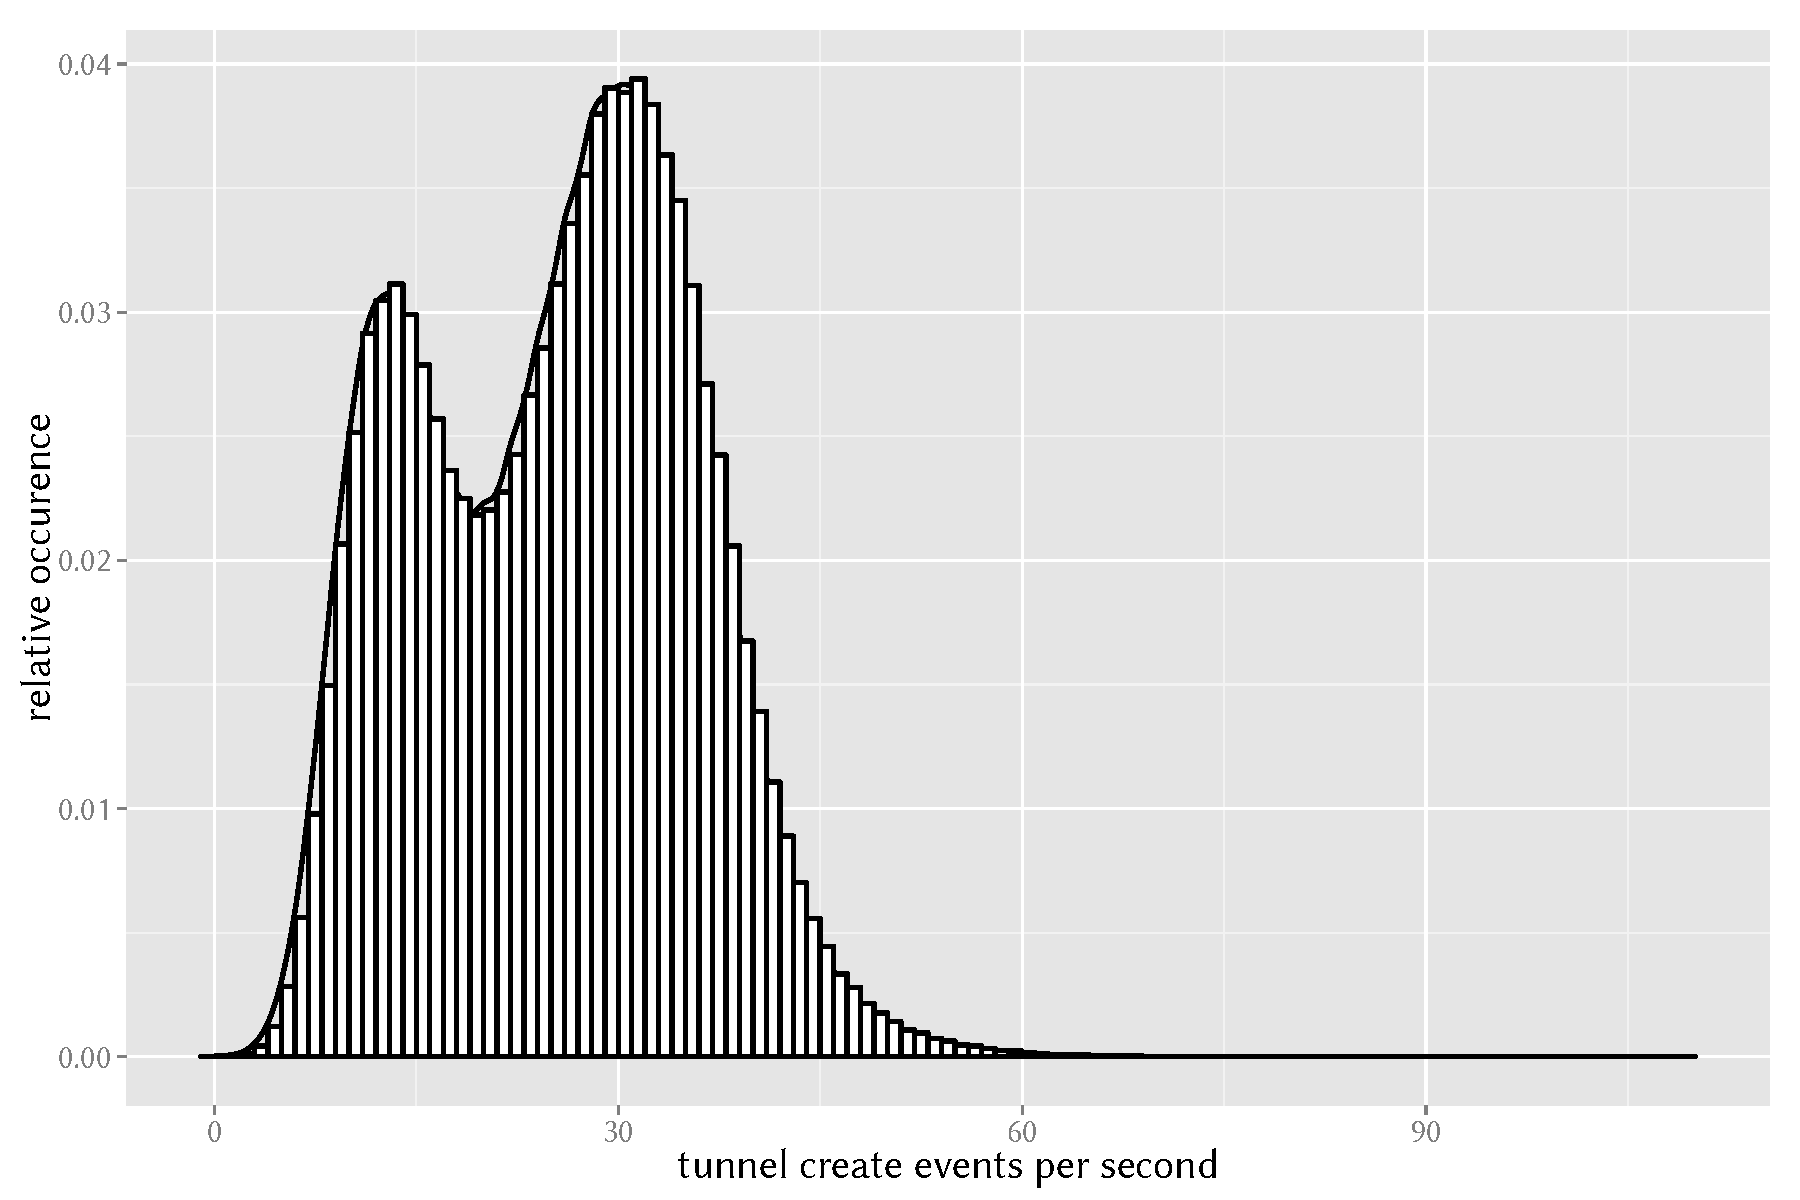
\includegraphics[width=6.5cm]{../../chapters/04-mobilenets/images/R-create-frequency.pdf}
		\end{column}
	\end{columns}

	\begin{itemize}
		\item Strong time of day dependence with busy hour in the early afternoon
	\end{itemize}
\end{frame}

\begin{frame}
	\frametitle{Tunnel Durations}
	\begin{center}
		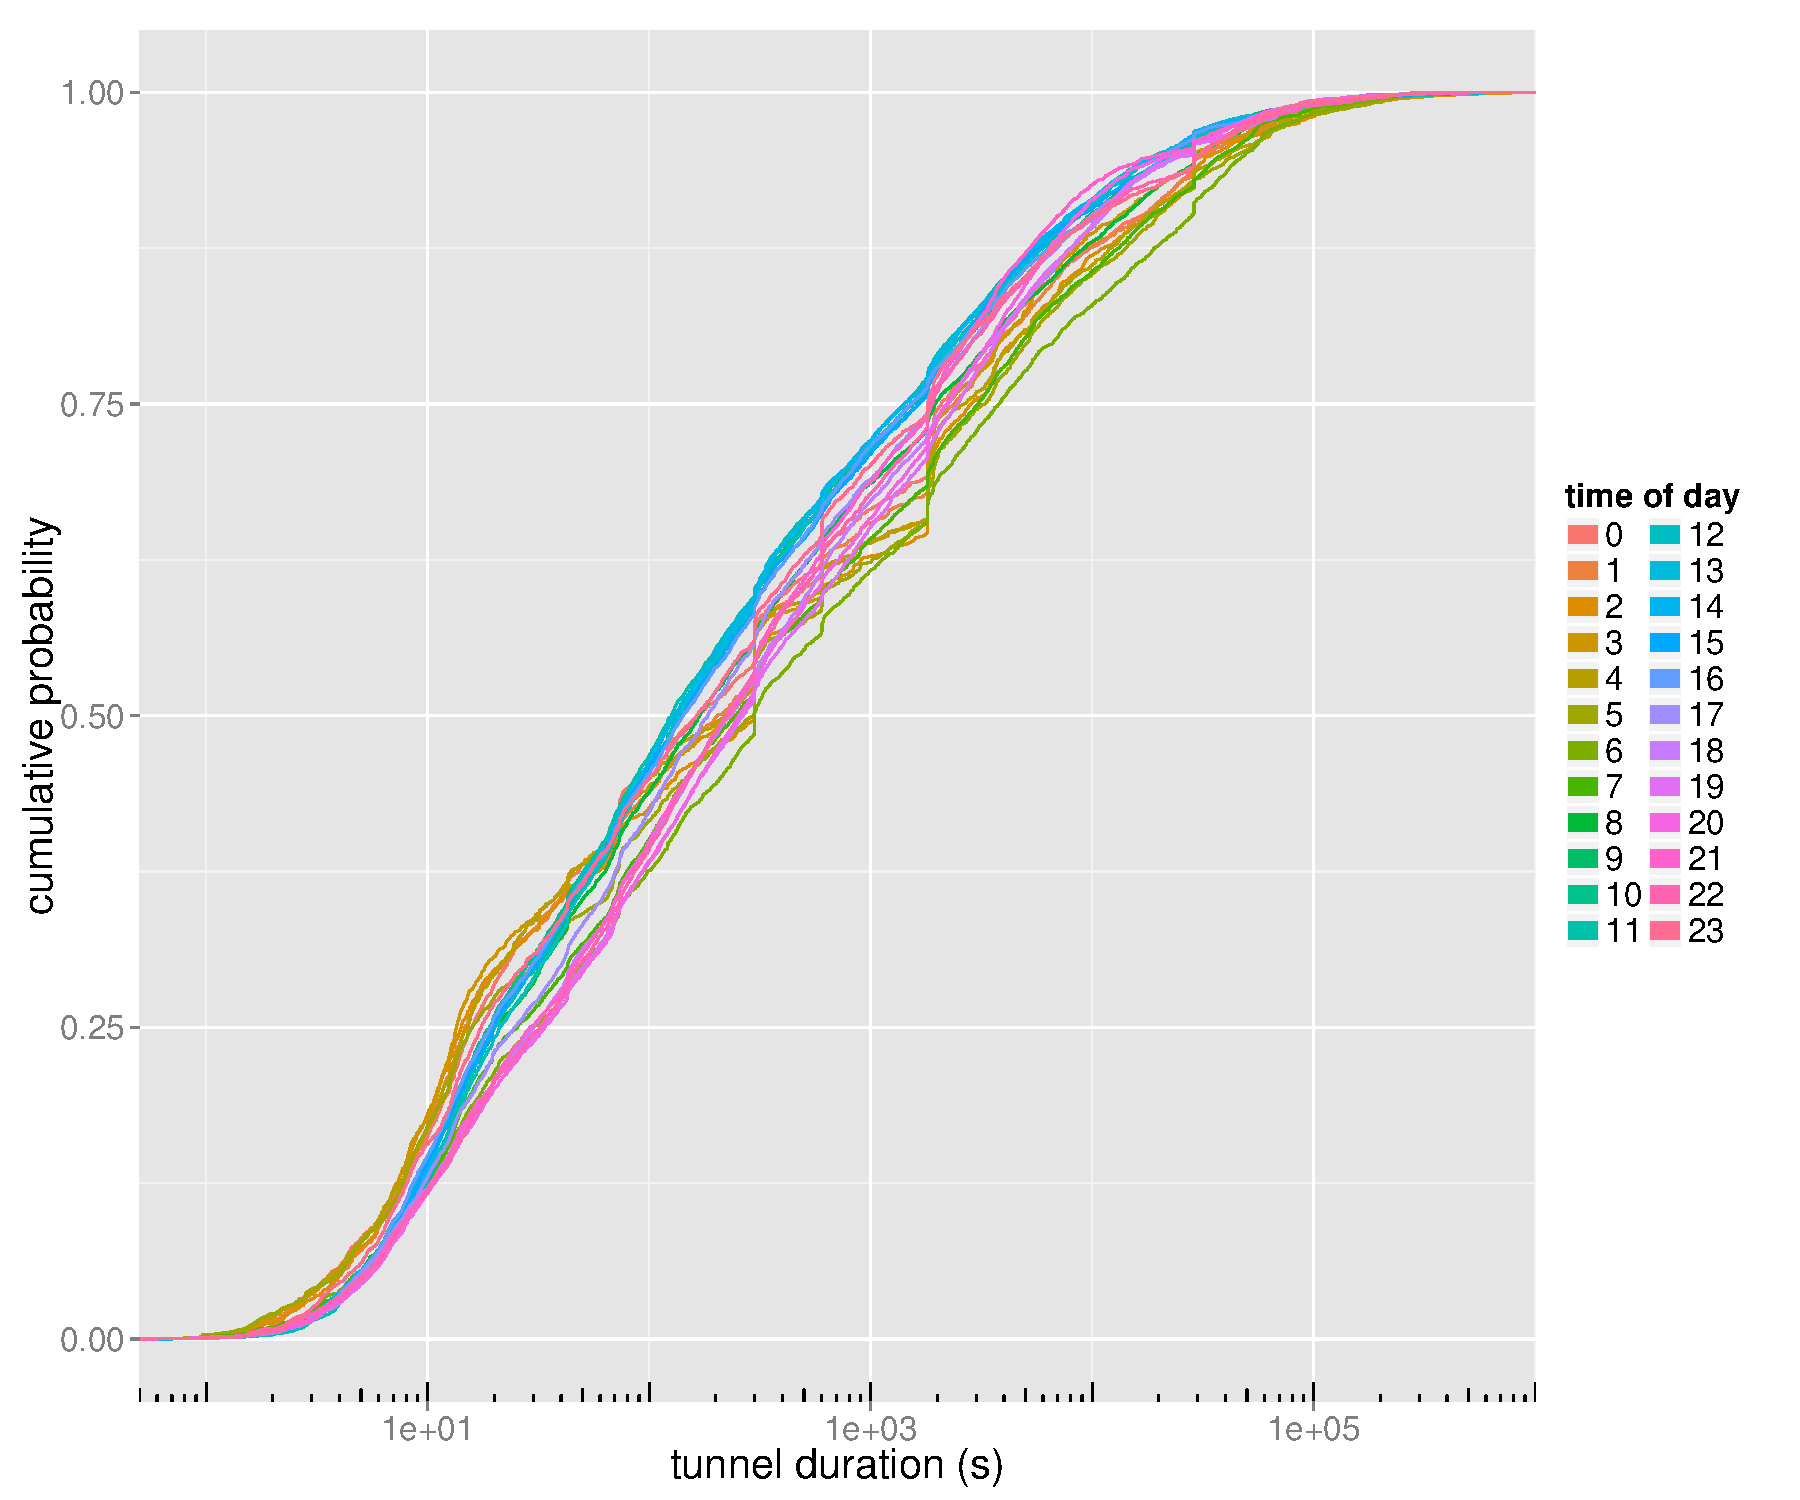
\includegraphics[height=5.5cm]{../../chapters/04-mobilenets/images/R-duration-timeofday-ecdf.pdf}
	\end{center}

	\begin{itemize}
		\item Only slight dependence on time of day
		\item Much stronger influence of user device type, OS, or network timers (not shown here)
	\end{itemize}
\end{frame}

%%%
\subsection{Models}
%%%


\begin{frame}
	\frametitle{Monolithic GGSN Queuing Model}
		\begin{center}
			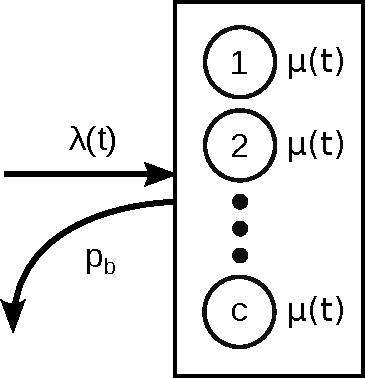
\includegraphics[height=3.5cm]{../../chapters/04-mobilenets/images/ggsn-monolithic.pdf}
		\end{center}

		\begin{itemize}
			\item Poisson tunnel arrival process with rate $\lambda(t)$, adjusted for the time of day
			\item GGSN can serve $n$ tunnels in parallel, limited by network/processing load and signaling/state overhead
			\item Tunnels have a duration of $\mu(t)$ with a general distribution
			\item If GGSN is full, reject new tunnels with blocking probability $p_b$
			\item[$\rightarrow$] Non-stationary Erlang loss model $M_t/G/n/0$ 
		\end{itemize}

\end{frame}

\begin{frame}
	\frametitle{Virtualized GGSN Queuing Model}
		\begin{center}
			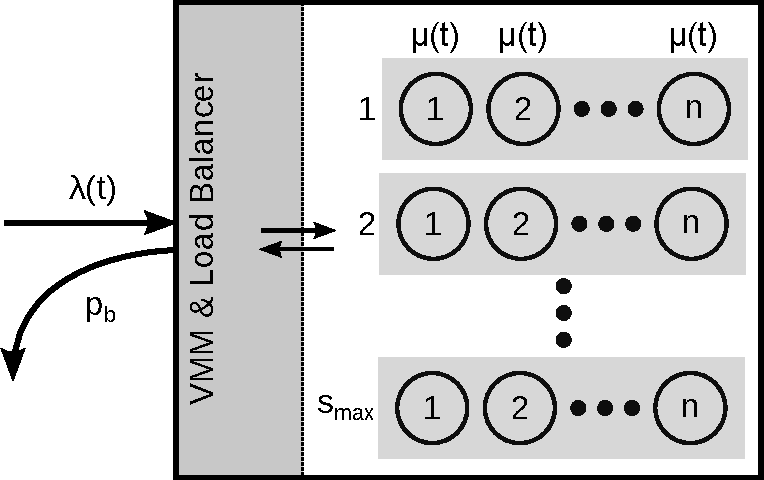
\includegraphics[height=3.5cm]{../../chapters/04-mobilenets/images/ggsn-virtualized.pdf}
		\end{center}

		\begin{itemize}
			\item Same arrival and serving time process, no queue
			\item Hypervisor distributes tunnels and starts on demand up to $s_{max}$ virtualized GGSN instances, each with capacity $m$
			%\item Up to $s_{max}$ instances with capacity of $m$ each
			%\item Instance count kept near actual system load (energy efficiency)
			\item Additional blocking when new instances are not switched on fast enough, or instance overhead if not shut down when unused
			\item System scales up (larger instances) and out (more instances)
		\end{itemize}
\end{frame}


%%%
\subsection{Queuing Simulation}
%%%


\begin{frame}
	\frametitle{Simulating the Model}

	\begin{itemize}
		\item No exact mathematical solution available for a $M_t/G/n/0$ model
		\item Use queuing simulation instead of stationary analysis
		\item SimPy3 based discrete event simulation\footnote{\url{https://github.com/fmetzger/ggsn-simulation}}
		\item One week simulated period, omitted startup phase, 10 repetitions
		\item Arrival process with exponential distributions fitted to dataset, four time of day slots ($\lambda=\{10.67,24.53,29.25,23.50\}$ before normalization)
		\item Tunnel duration CDF fitted with a rational function
		%\item Simple hypervisor instance start logic: always keep at least one active free instance in reserve
		\item Scenario variable parameters: $n$, $m$, and $s_{max}$
		\item Evaluate and compare both models based on
		\begin{itemize}
			\item Blocking probability
			\item resource and instance usage
		\end{itemize}
	\end{itemize}

\end{frame}

\begin{frame}
	\frametitle{Blocking Probability}

	\begin{center}
		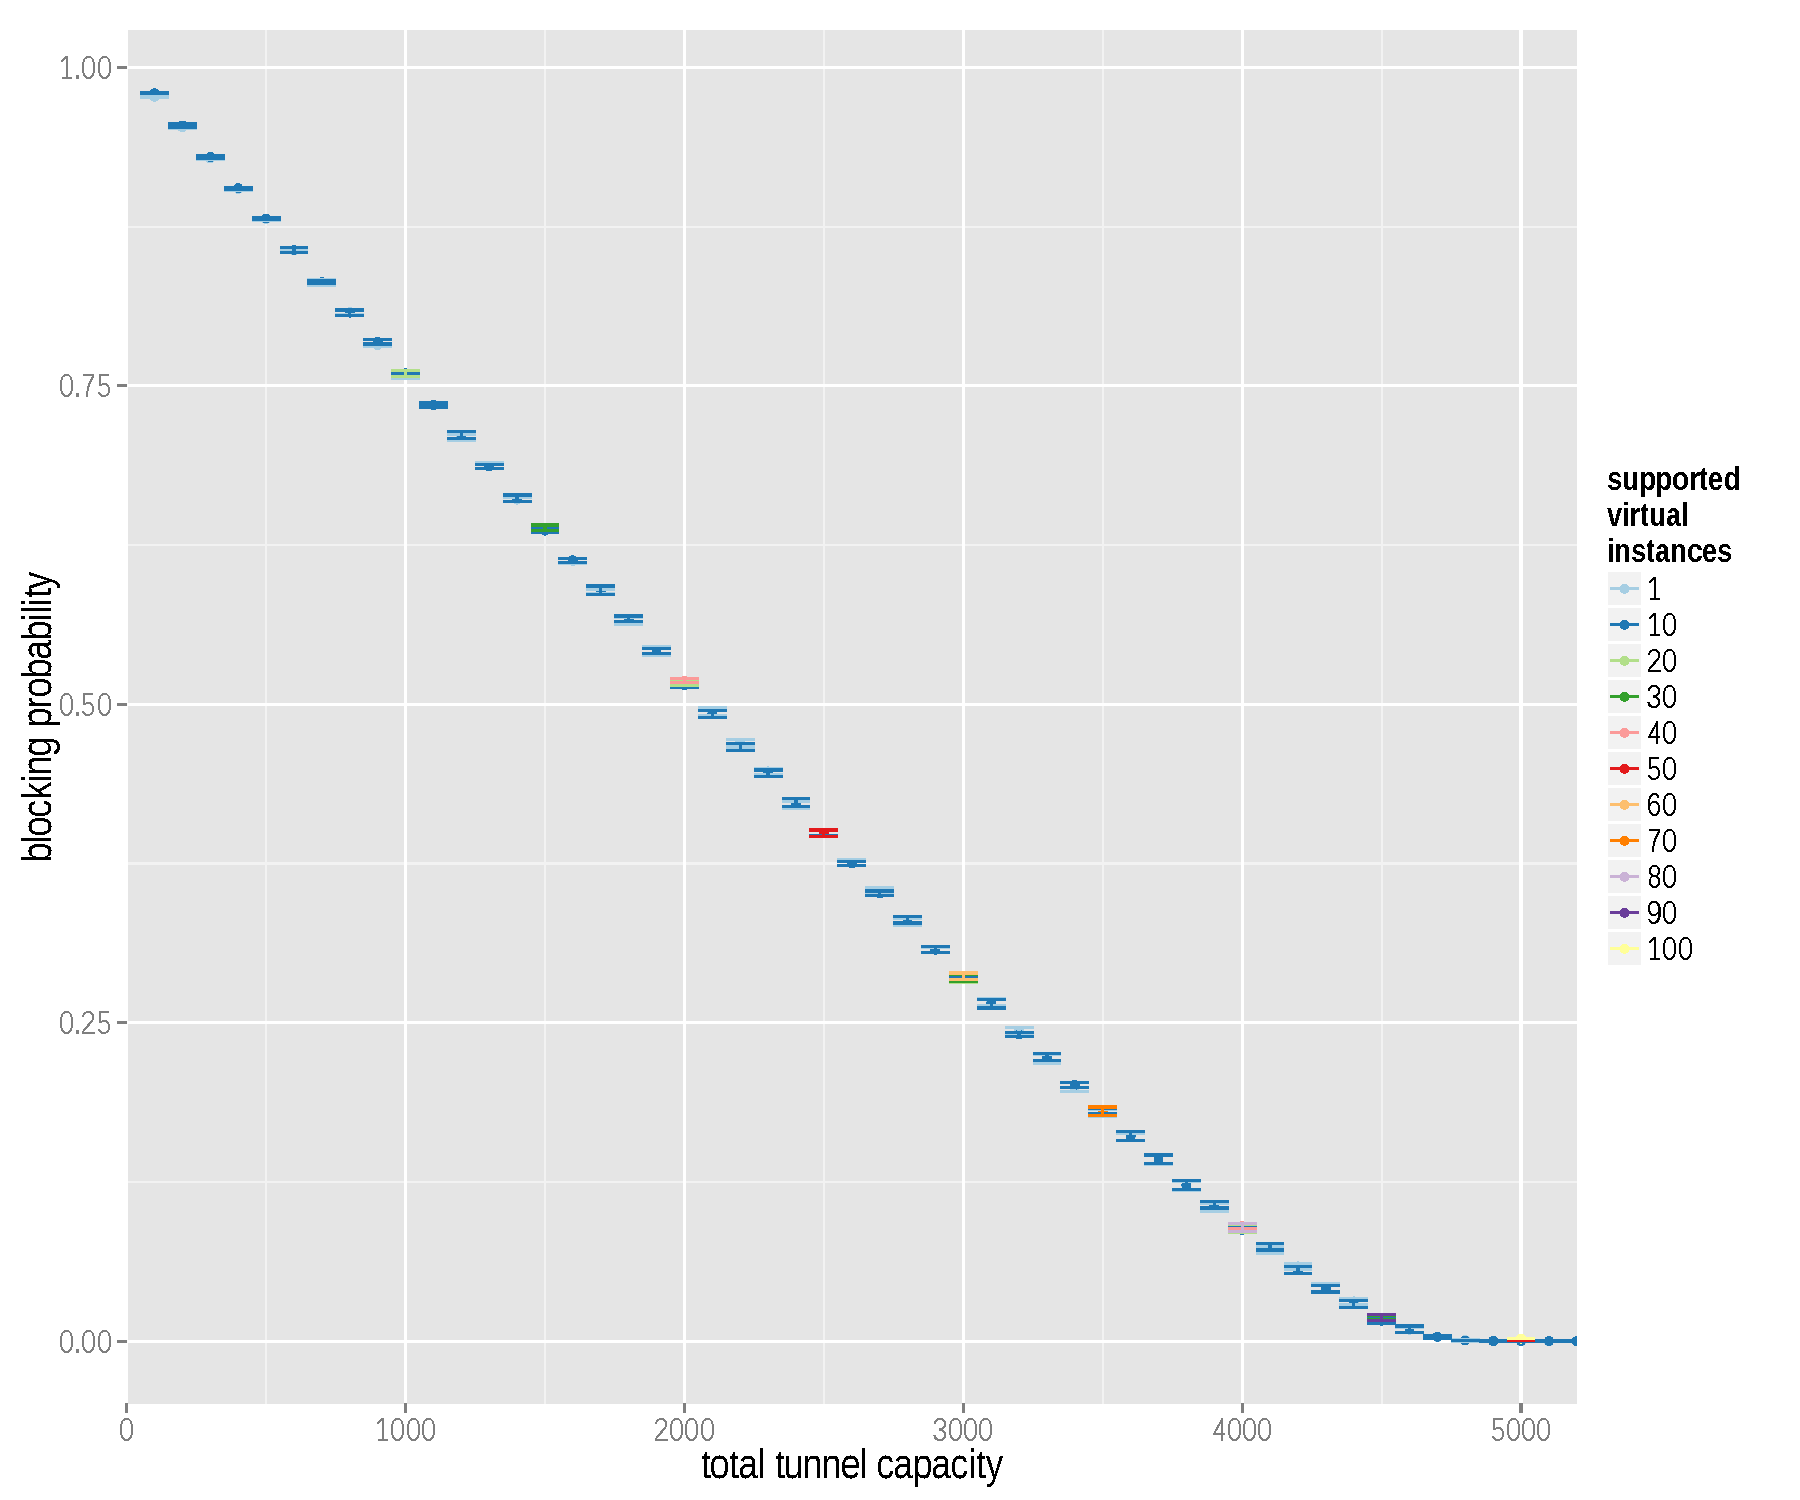
\includegraphics[height=5.5cm]{../../chapters/04-mobilenets/images/R-virtualized-blocking.pdf}
	\end{center}

	\begin{itemize}
		\item Monolithic and virtualized GGSN scale equally with supported tunnels
		\item Negligible to no impact on $p_B$ if virtualized model is scaled by tuning $s_{max}$ instead of $m$
	\end{itemize}
\end{frame}




\begin{frame}
	\frametitle{Virtualized GGSN Resource Usage}

	\begin{center}
		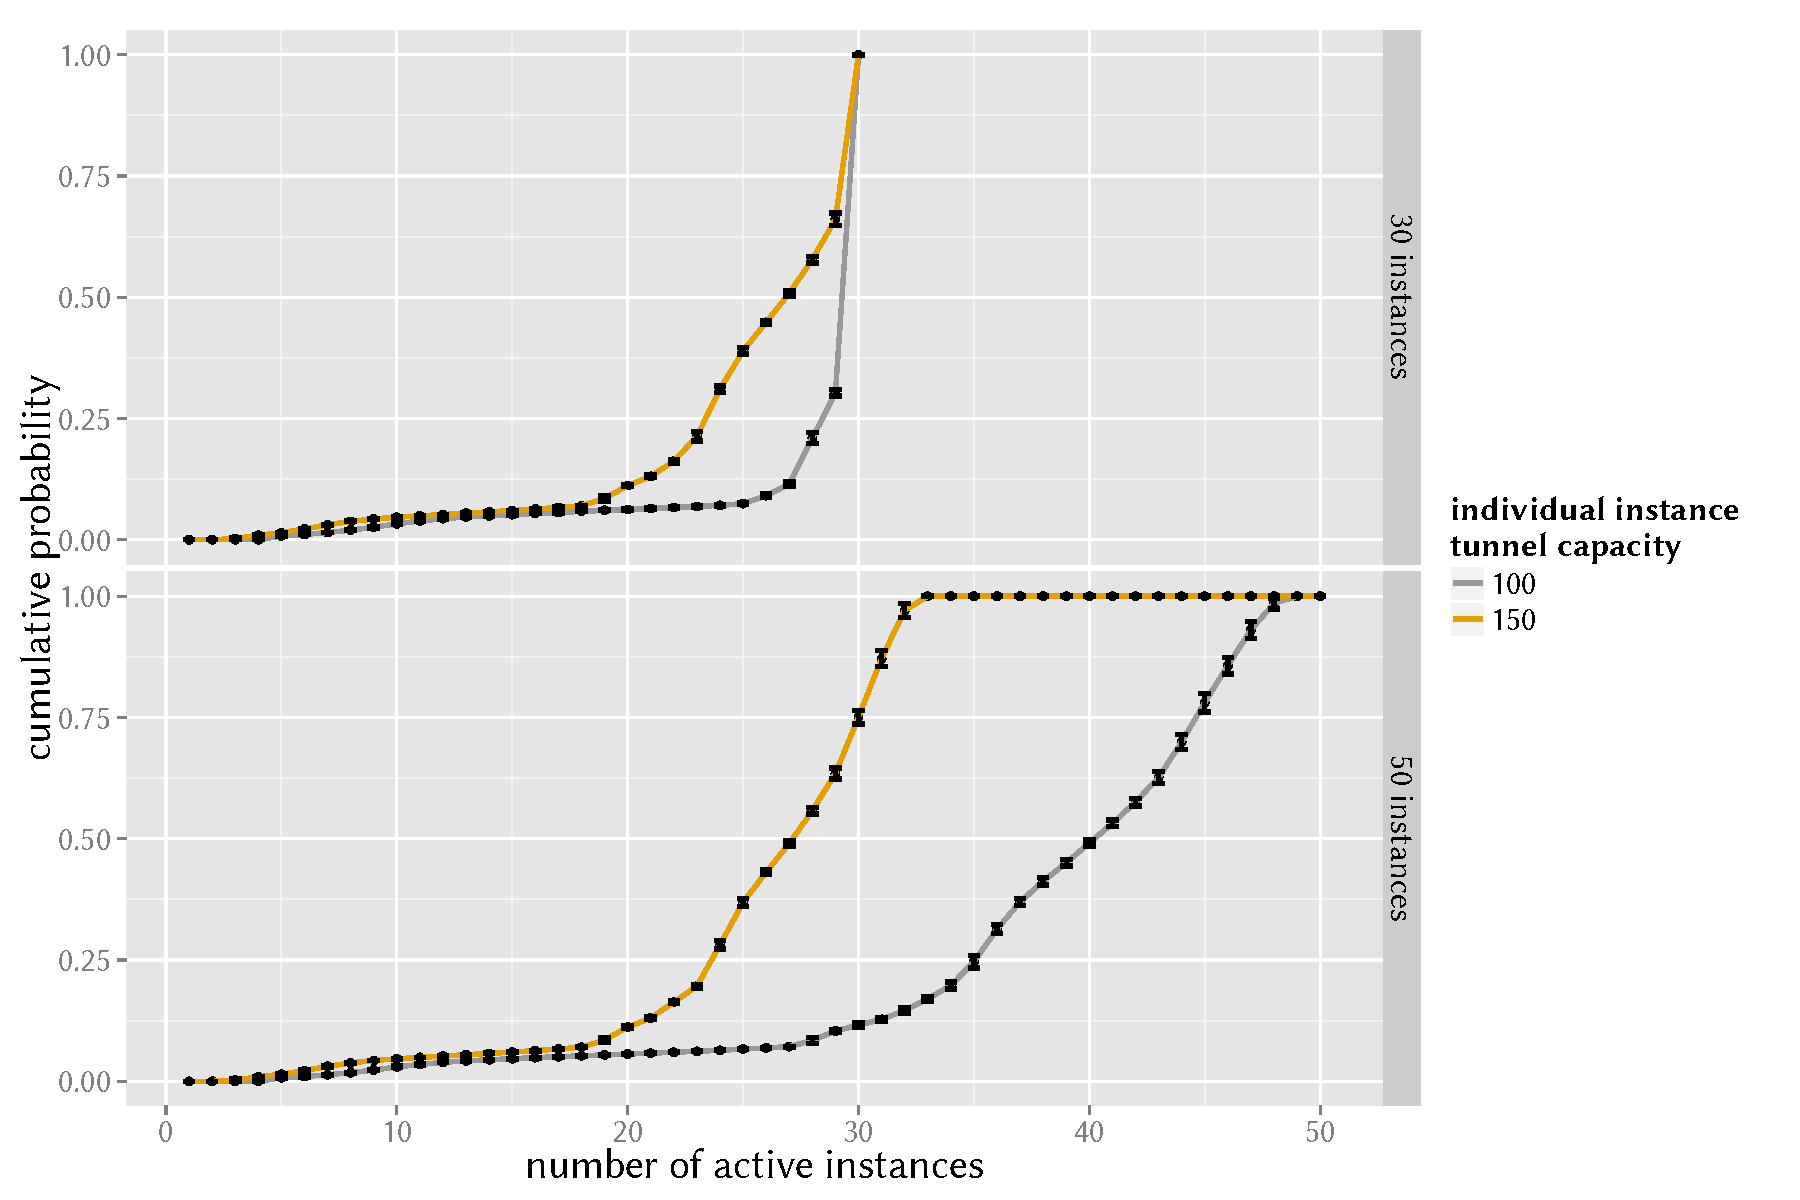
\includegraphics[height=5cm]{../../chapters/04-mobilenets/images/R-virtualized-instanceuse.pdf}
	\end{center}

	\begin{itemize}
		%\item System scales both up (tunnels/instance) and out (instances)
		\item Unused instances can be shut down for increased energy efficiency compared to monolithic model
	\end{itemize}
\end{frame}



%%%%%%%%%%%%%%%%%%%%%%%%%%%%%%%%%%%%%%%%%%%%%%%%%%%%%%%%%%%%%%%%%%%%%%%%%%%%%%%%
\section{Influences}
%%%

\begin{frame}
	\frametitle{Introduction}
\end{frame}






%%%%%%%%%%%%%%%%%%%%%%%%%%%%%%%%%%%%%%%%%%%%%%%%%%%%%%%%%%%%%%%%%%%%%%%%%%%%%%%%
\section{Measuring Mobile Reliable Streaming}
%%%

\begin{frame}
	\frametitle{Introduction}
\end{frame}





%%%%%%%%%%%%%%%%%%%%%%%%%%%%%%%%%%%%%%%%%%%%%%%%%%%%%%%%%%%%%%%%%%%%%%%%%%%%%%%%
\section{Conclusions}
%%%

\begin{frame}
	\frametitle{Conclusion}

	\begin{itemize}
		\item Investigated tunnel properties in core network dataset

		\begin{itemize}
			\item Non-stationary Poisson arrivals
			\item Tunnel duration with general distribution
		\end{itemize}

		\item Erlang loss models for tunnel load at a mobile core network's GGSN
		\begin{itemize}
			\item Monolithic GGSN representing today's makeup
			\item Virtualized GGSN proposal with improved scalability and efficiency
		\end{itemize}

		\item Simulative evaluation of the model

		\item Enable mobile network dimensioning based on tunnel blocking rate instead of only user traffic volume


	\end{itemize}

\end{frame}

%%%%%%%%%%%%%%%%%%%%%%%%%%%%%%%%%%%%%%%%%%%%%%%%%%%%%%%%%%%%%%%%%%%%%%%%%%%%%%%%
\section*{}
%%
\begin{frame}
	\frametitle{Thanks!}

	\centering
		\Large Questions?
\end{frame}




%%%%%%%%%%%%%%%%%%%%%%%%%%%%%%%%%%%%%%%%%%%%%%%%%%%%%%%%%%%%%%%%%%%%%%%%%%%%%%%%
\section{References}
\begin{frame}[t,allowframebreaks]
	\frametitle{References}
	\printbibliography
\end{frame}





%%%%%%%%%%%%%%%%%%%%%%%%%%%%%%%%%%%%%%%%%%%%%%%%%%%%%%%%%%%%%%%%%%%%%%%%%%%%%%%%
\appendix
\newcounter{finalframe}
\setcounter{finalframe}{\value{framenumber}}

\begin{frame}
\end{frame}




\begin{frame}
	\frametitle{}
	\begin{center}
		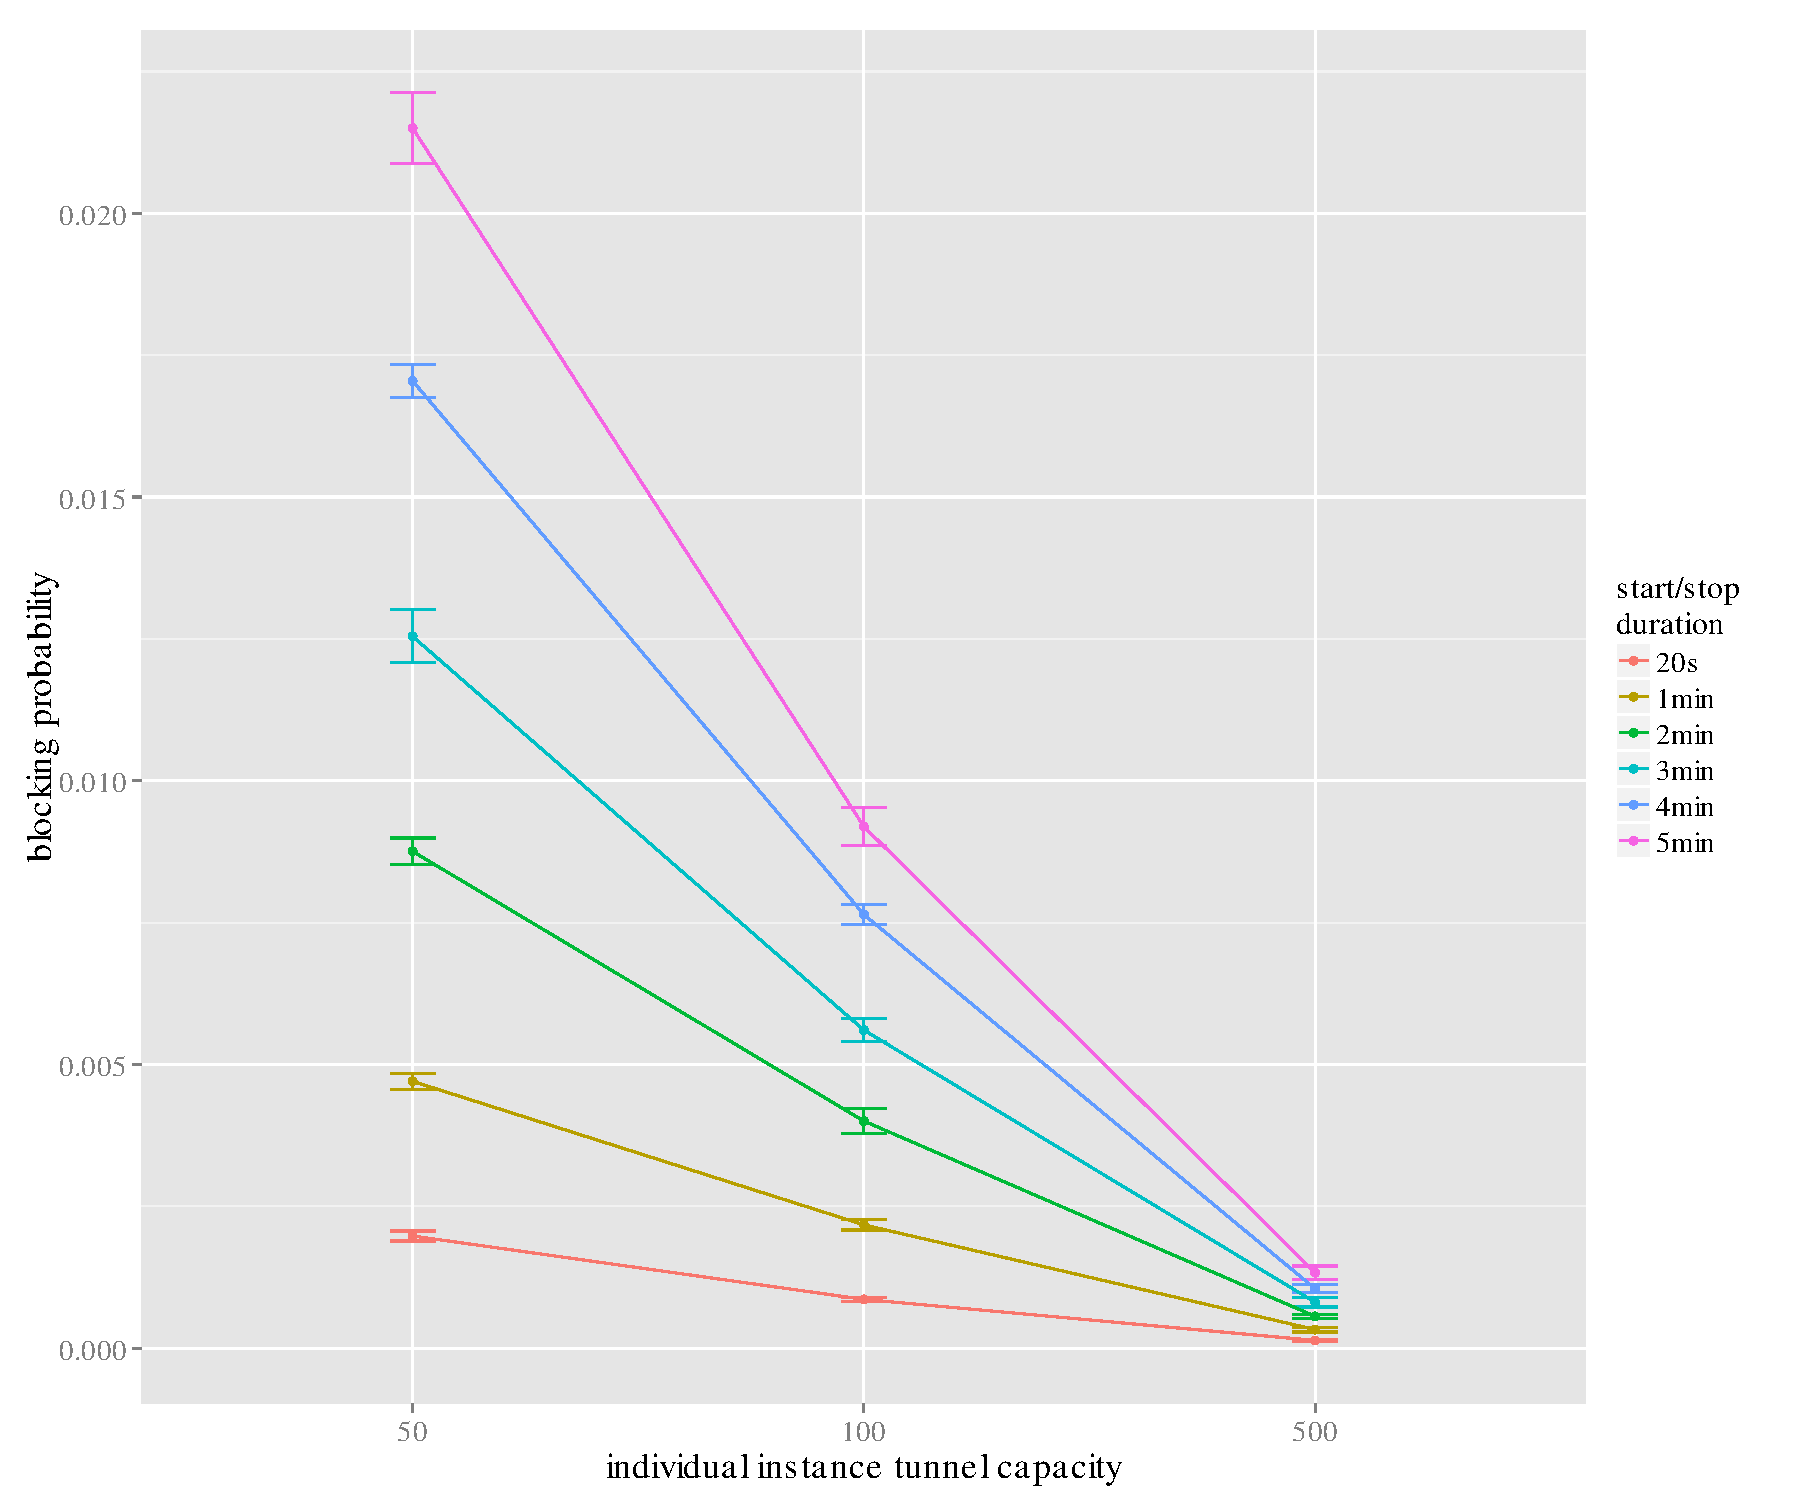
\includegraphics[height=7cm]{../../chapters/04-mobilenets/images/compare-maxinstances-block.pdf}
	\end{center}
\end{frame}


\begin{frame}
	\frametitle{Exponential Arrival Process Fits}

	\begin{center}
		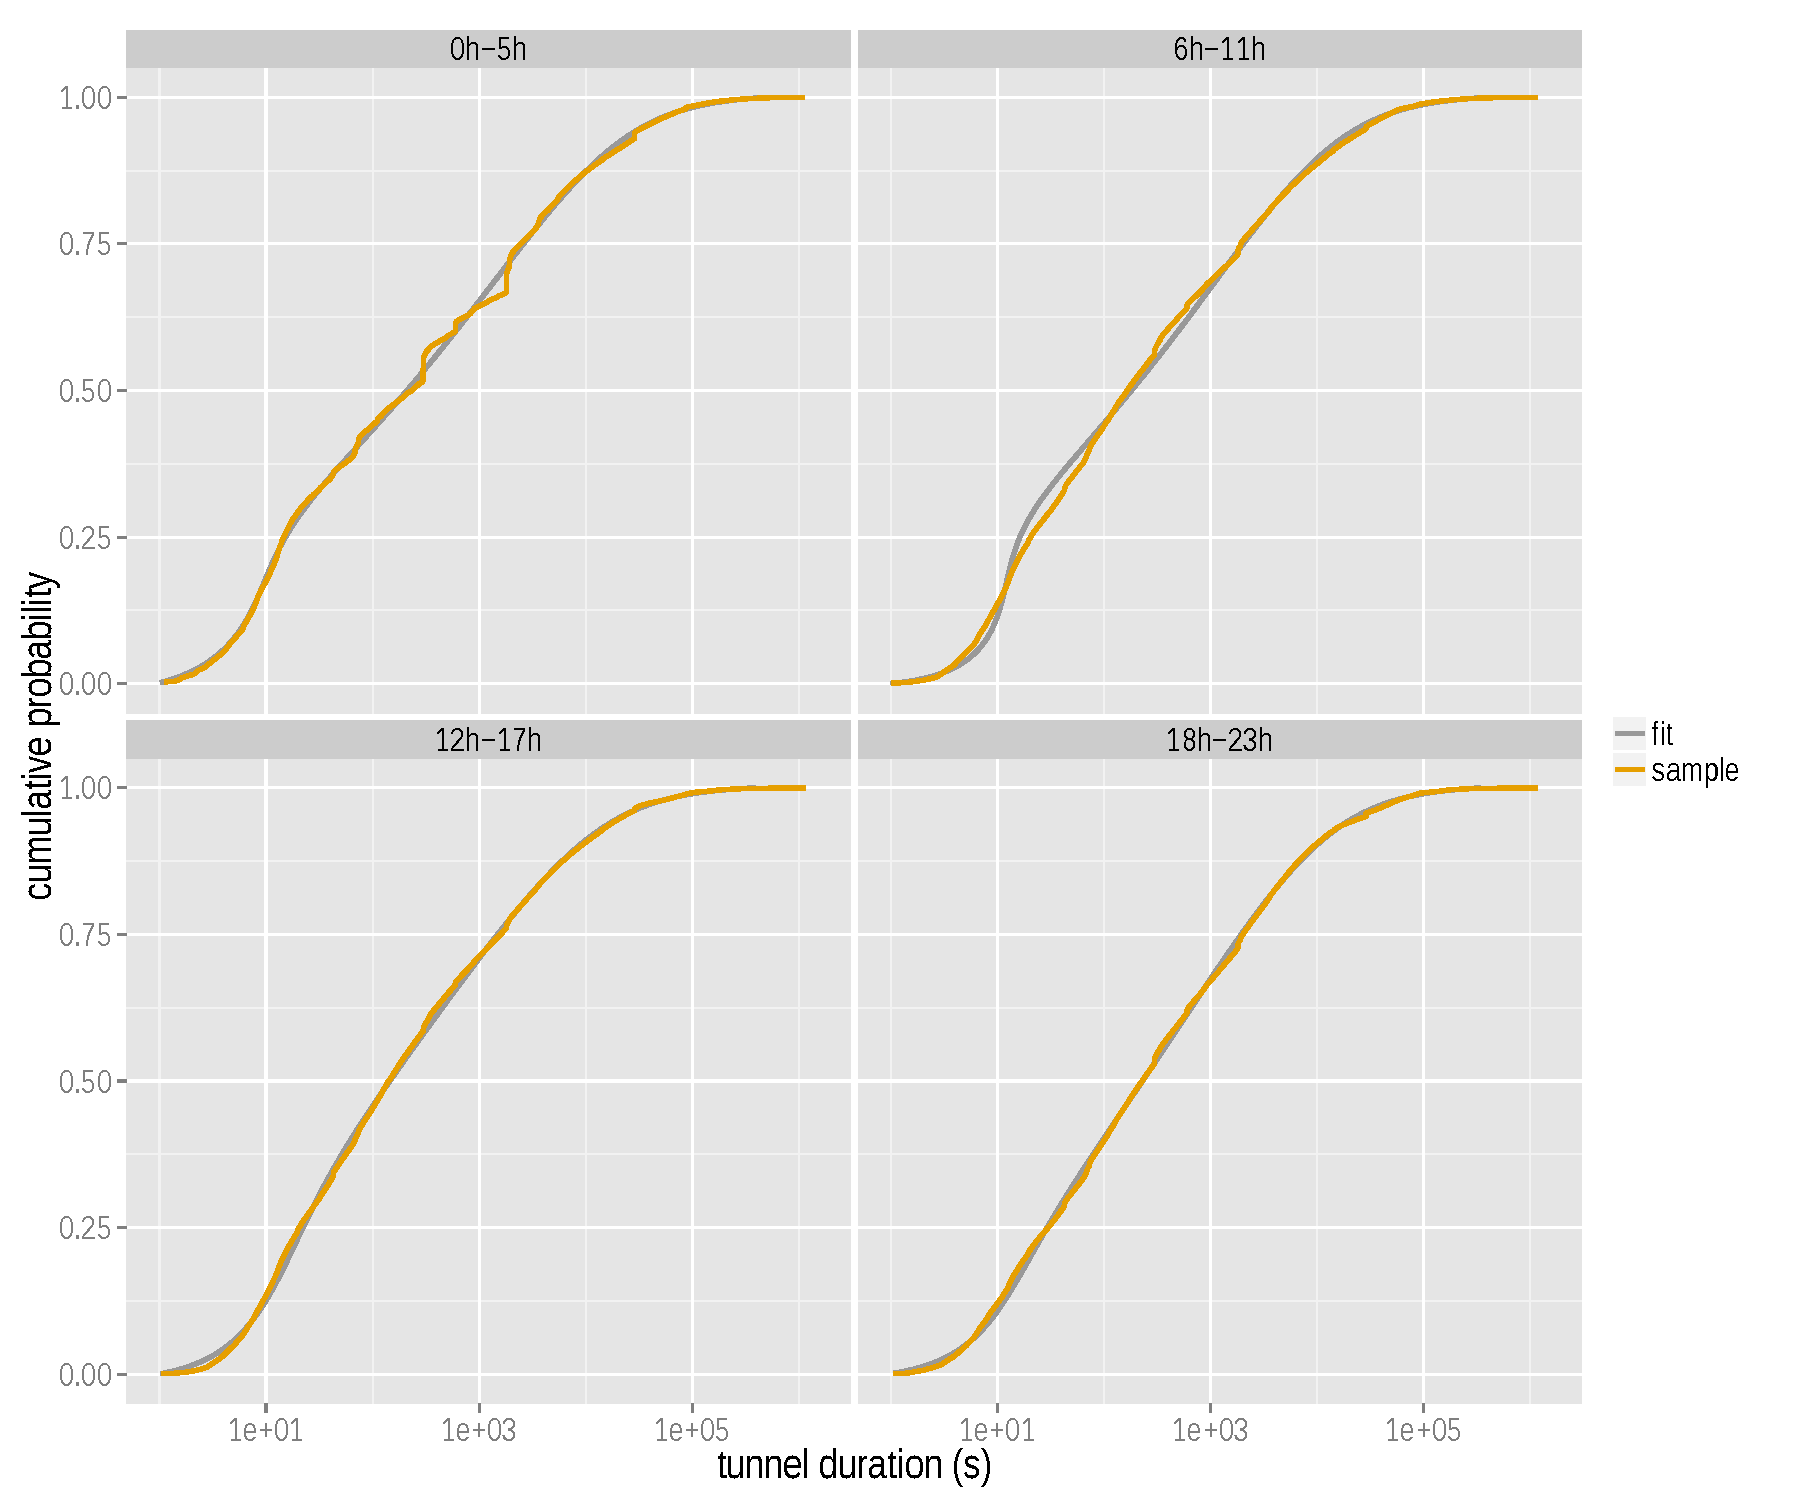
\includegraphics[height=7.5cm]{../../chapters/04-mobilenets/images/R-duration-fit-cdf-facets.pdf}
	\end{center}
\end{frame}

\begin{frame}
	\frametitle{Serving Time Rational Functions Fit}

	\begin{center}
		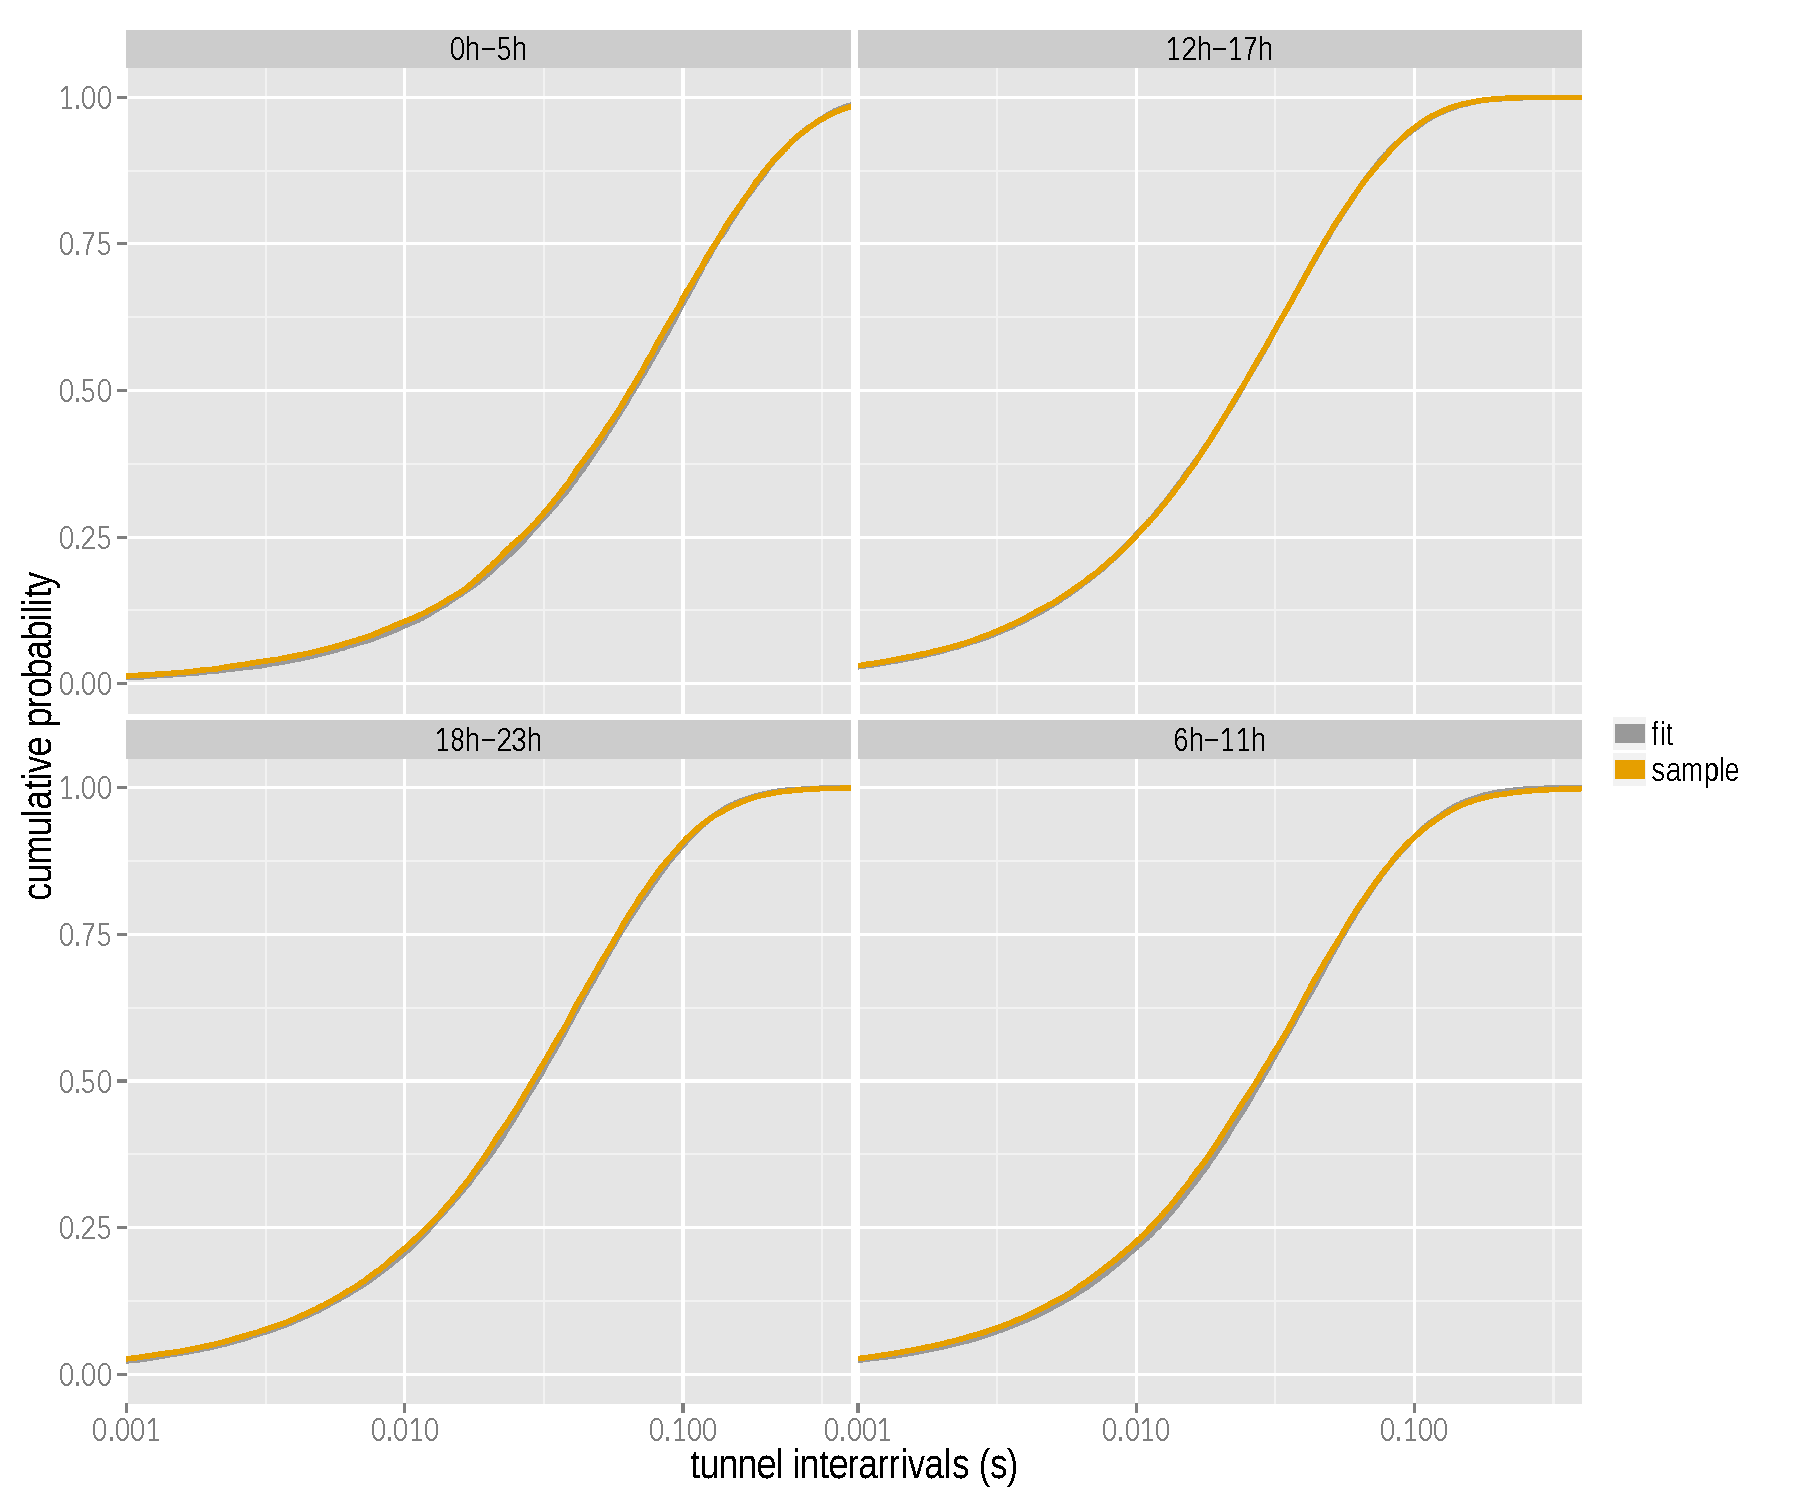
\includegraphics[height=7.5cm]{../../chapters/04-mobilenets/images/R-IAT-active-fit-cdf-facets.pdf}
	\end{center}
\end{frame}

\begin{frame}
	\frametitle{Scaling Up or Out with a Virtualized GGSN}
	
	\begin{center}
		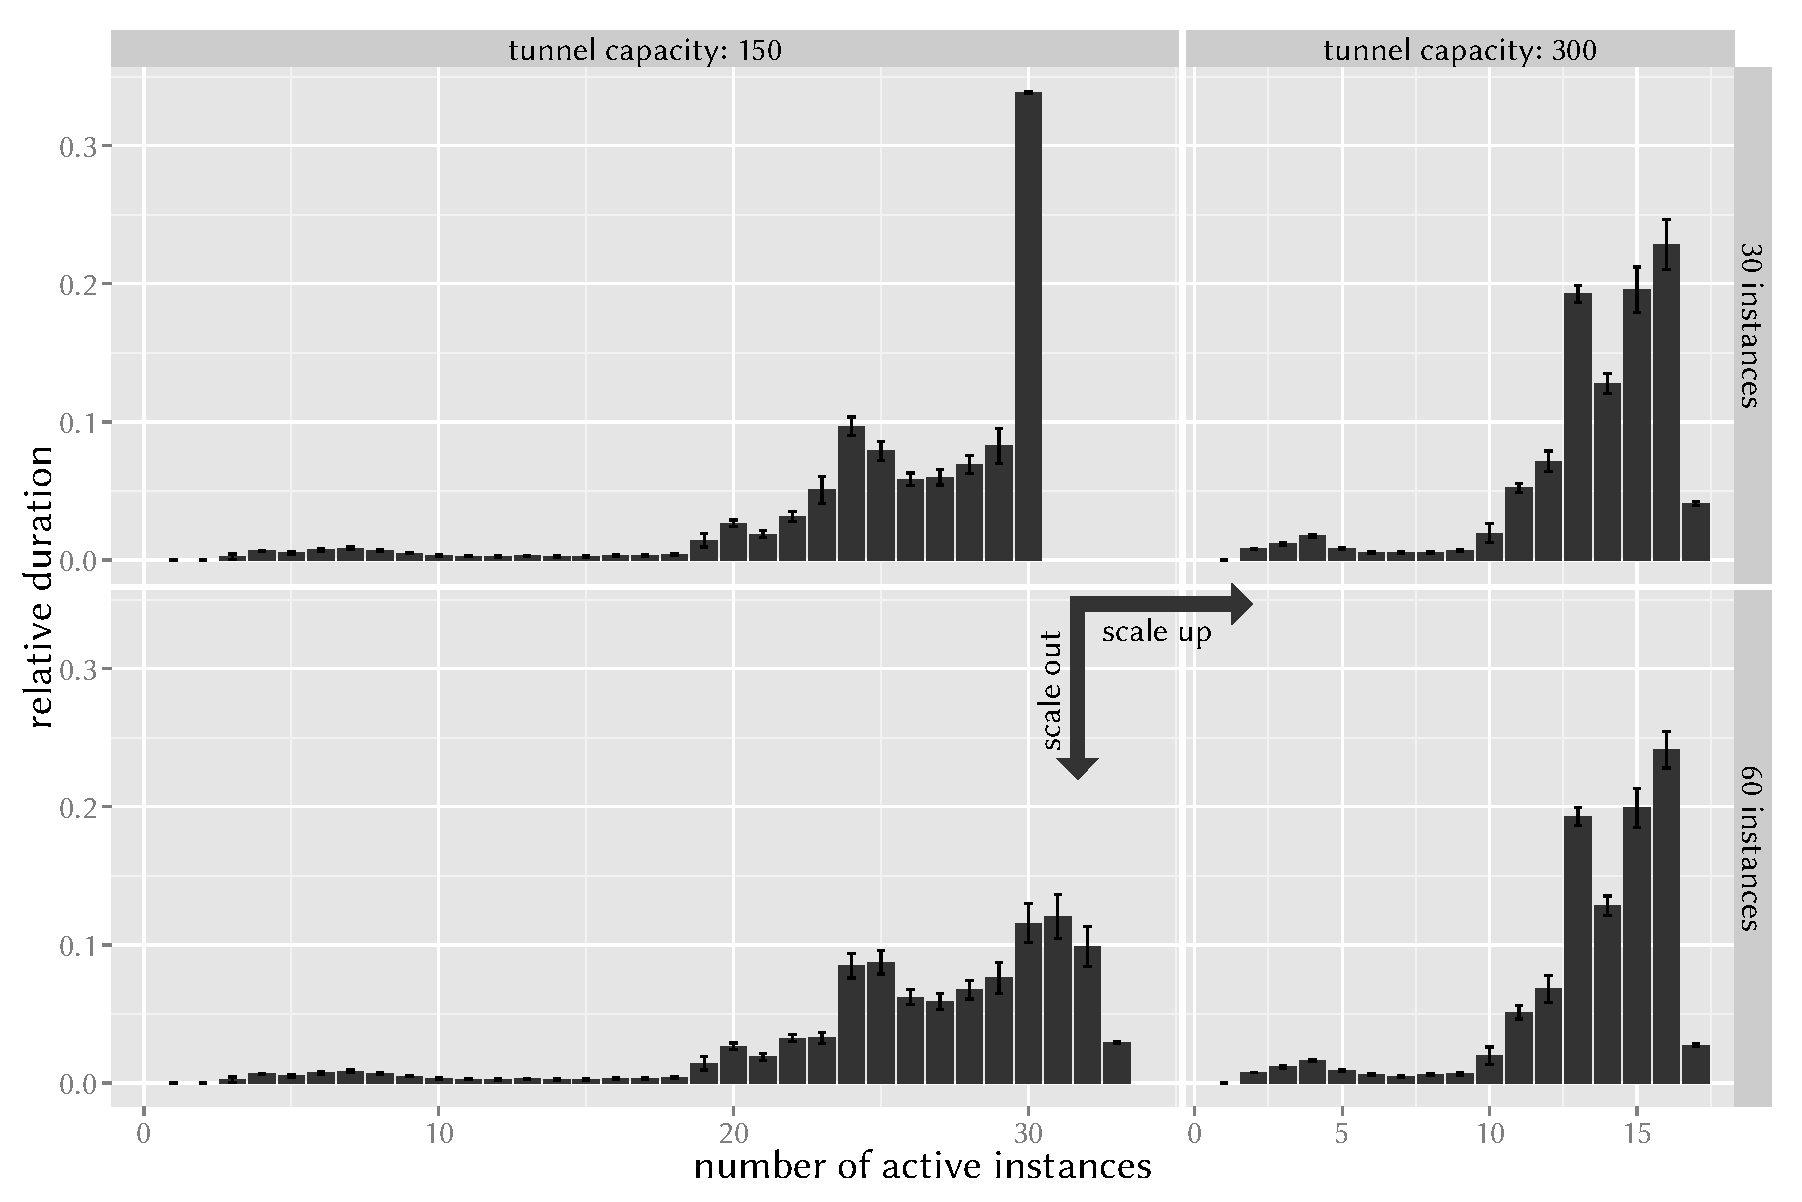
\includegraphics[height=7cm]{../../chapters/04-mobilenets/images/R-virtualized-instanceuse-barplot.pdf}
	\end{center}
\end{frame}

\begin{frame}
	\frametitle{Queuing Models}

	\begin{center}
		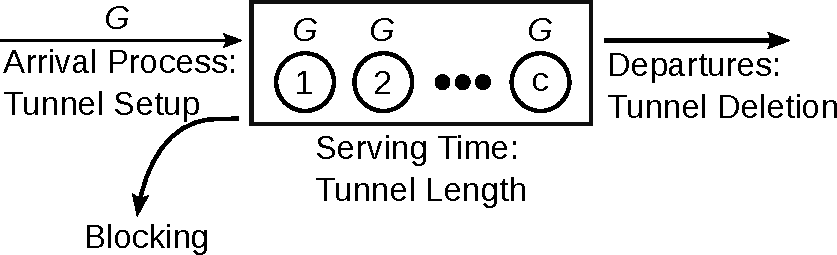
\includegraphics[height=2cm]{../../chapters/04-mobilenets/images/GGn-model.pdf}
	\end{center}

	Described by Kendall's Notation $A/S/c/q$
	\begin{itemize}
	\item Distribution of the arrival process $A$
		% \begin{itemize}
		% 	\item Poisson arrivals, memoryless
		% 	\item Markov chain model
		% \end{itemize}
	\item Distribution of the serving time $S$
	\item Number of Servers $c$
	\item Queue Length $q$
	\begin{itemize}
		\item $q=\infty$ no loss will occur
		\item $0$ loss/blocking system, no queue
	\end{itemize}
	\item Evaluate
		\begin{itemize}
			\item Average queue length and server occupation
			\item Blocking probability
		\end{itemize}
	\end{itemize}
\end{frame}

\setcounter{framenumber}{\value{finalframe}}

\end{document}



% \begin{frame}
% 	\frametitle{The Dataset}

% 	\begin{itemize}
% 		\item one week long passive measurements in the core network of a operator (METAWIN, April 2011)
% 		\item 2.2Bn anonymized user traffic records, 410M GTP tunnel management messages
% 	\end{itemize}

% 	Evaluated properties important for the model
% 	\begin{itemize}
% 		\item arrival rate of new tunnels
% 		\item duration of tunnels
% 		\item and diurnal influences on them
% 	\end{itemize}
% \end{frame}

% \begin{frame}
% 	\frametitle{Fitting Distributions to the Data}
% 	\begin{itemize}
% 		\item Data preparation with mysql \& python
% 		\begin{itemize}
% 			\item Fetch CREATE and DELETE from db
% 			\item Calculate tunnel IAT and durations
% 		\end{itemize}
% 		\item Statistical analysis and fitting using R/fitdistrplus/MASS
% 		\begin{itemize}
% 			\item $1\%$ random sampling of the data
% 			\item Distribution parameter estimation by closed formula matching of theoretical and observed means and variances (Method of Moments Estimation)
% 			\item Testing goodness of the fit
% 				\begin{itemize}
% 					\item Pearson's $\chi^2$-test
% 					\item Kolmogorov-Smirnov $d = \max|F_n(x)-F(x)|$
% 					\item Visually
% 					\item ANOVA
% 				\end{itemize}
% 		\end{itemize}
% 	\end{itemize}
% \end{frame}


